\documentclass[
%	aspectratio=169
]{beamer}
\usetheme{jdpg}


%\usepackage{etex}
\usepackage[utf8]{inputenc}
%\usepackage[T1]{fontenc}
%\usepackage{lmodern}
\usepackage[english,ngerman]{babel}
%\usepackage{textcomp}
\usepackage{enumitem}
\usepackage{microtype}
\usepackage{amsthm}
\usepackage{amssymb}
\usepackage{amsmath}
\usepackage{graphicx}
\usepackage{siunitx}
%\usepackage{url}
\newcommand\euro{{\sffamily C%
 \makebox[0pt][l]{\kern-.70em\mbox{--}}%
 \makebox[0pt][l]{\kern-.68em\raisebox{.25ex}{--}}}}
 

\hypersetup{
	pdfauthor={Martin Wengenmayr},
	pdftitle={Bundesweites},
	pdfpagemode=FullScreen,
}
%\pgfdeclareimage[height==\verb=1cm]{logo}{logo.eps}
%\logo{\pgfuseimage{logo}}

\setitemize{label={\color{jblue}\textbullet}}
%\renewcommand{\labelitemi}{{\color{lightgray}\textbullet}}


\title[Bundesweites]{Workshop Bundesweite Veranstaltungen}
%\subtitle{Eine Kurzvorstellung}
\author[Martin \& Monique]{Martin Wengenmayr \& Monique Honsa}
\date{\today}
\institute[]{A-Team Promotion}

\begin{document}

\maketitle

\begin{frame}{}
 \tableofcontents
\end{frame}

\begin{frame}{Gehirnsturm I}
  \begin{figure}
   \centering
   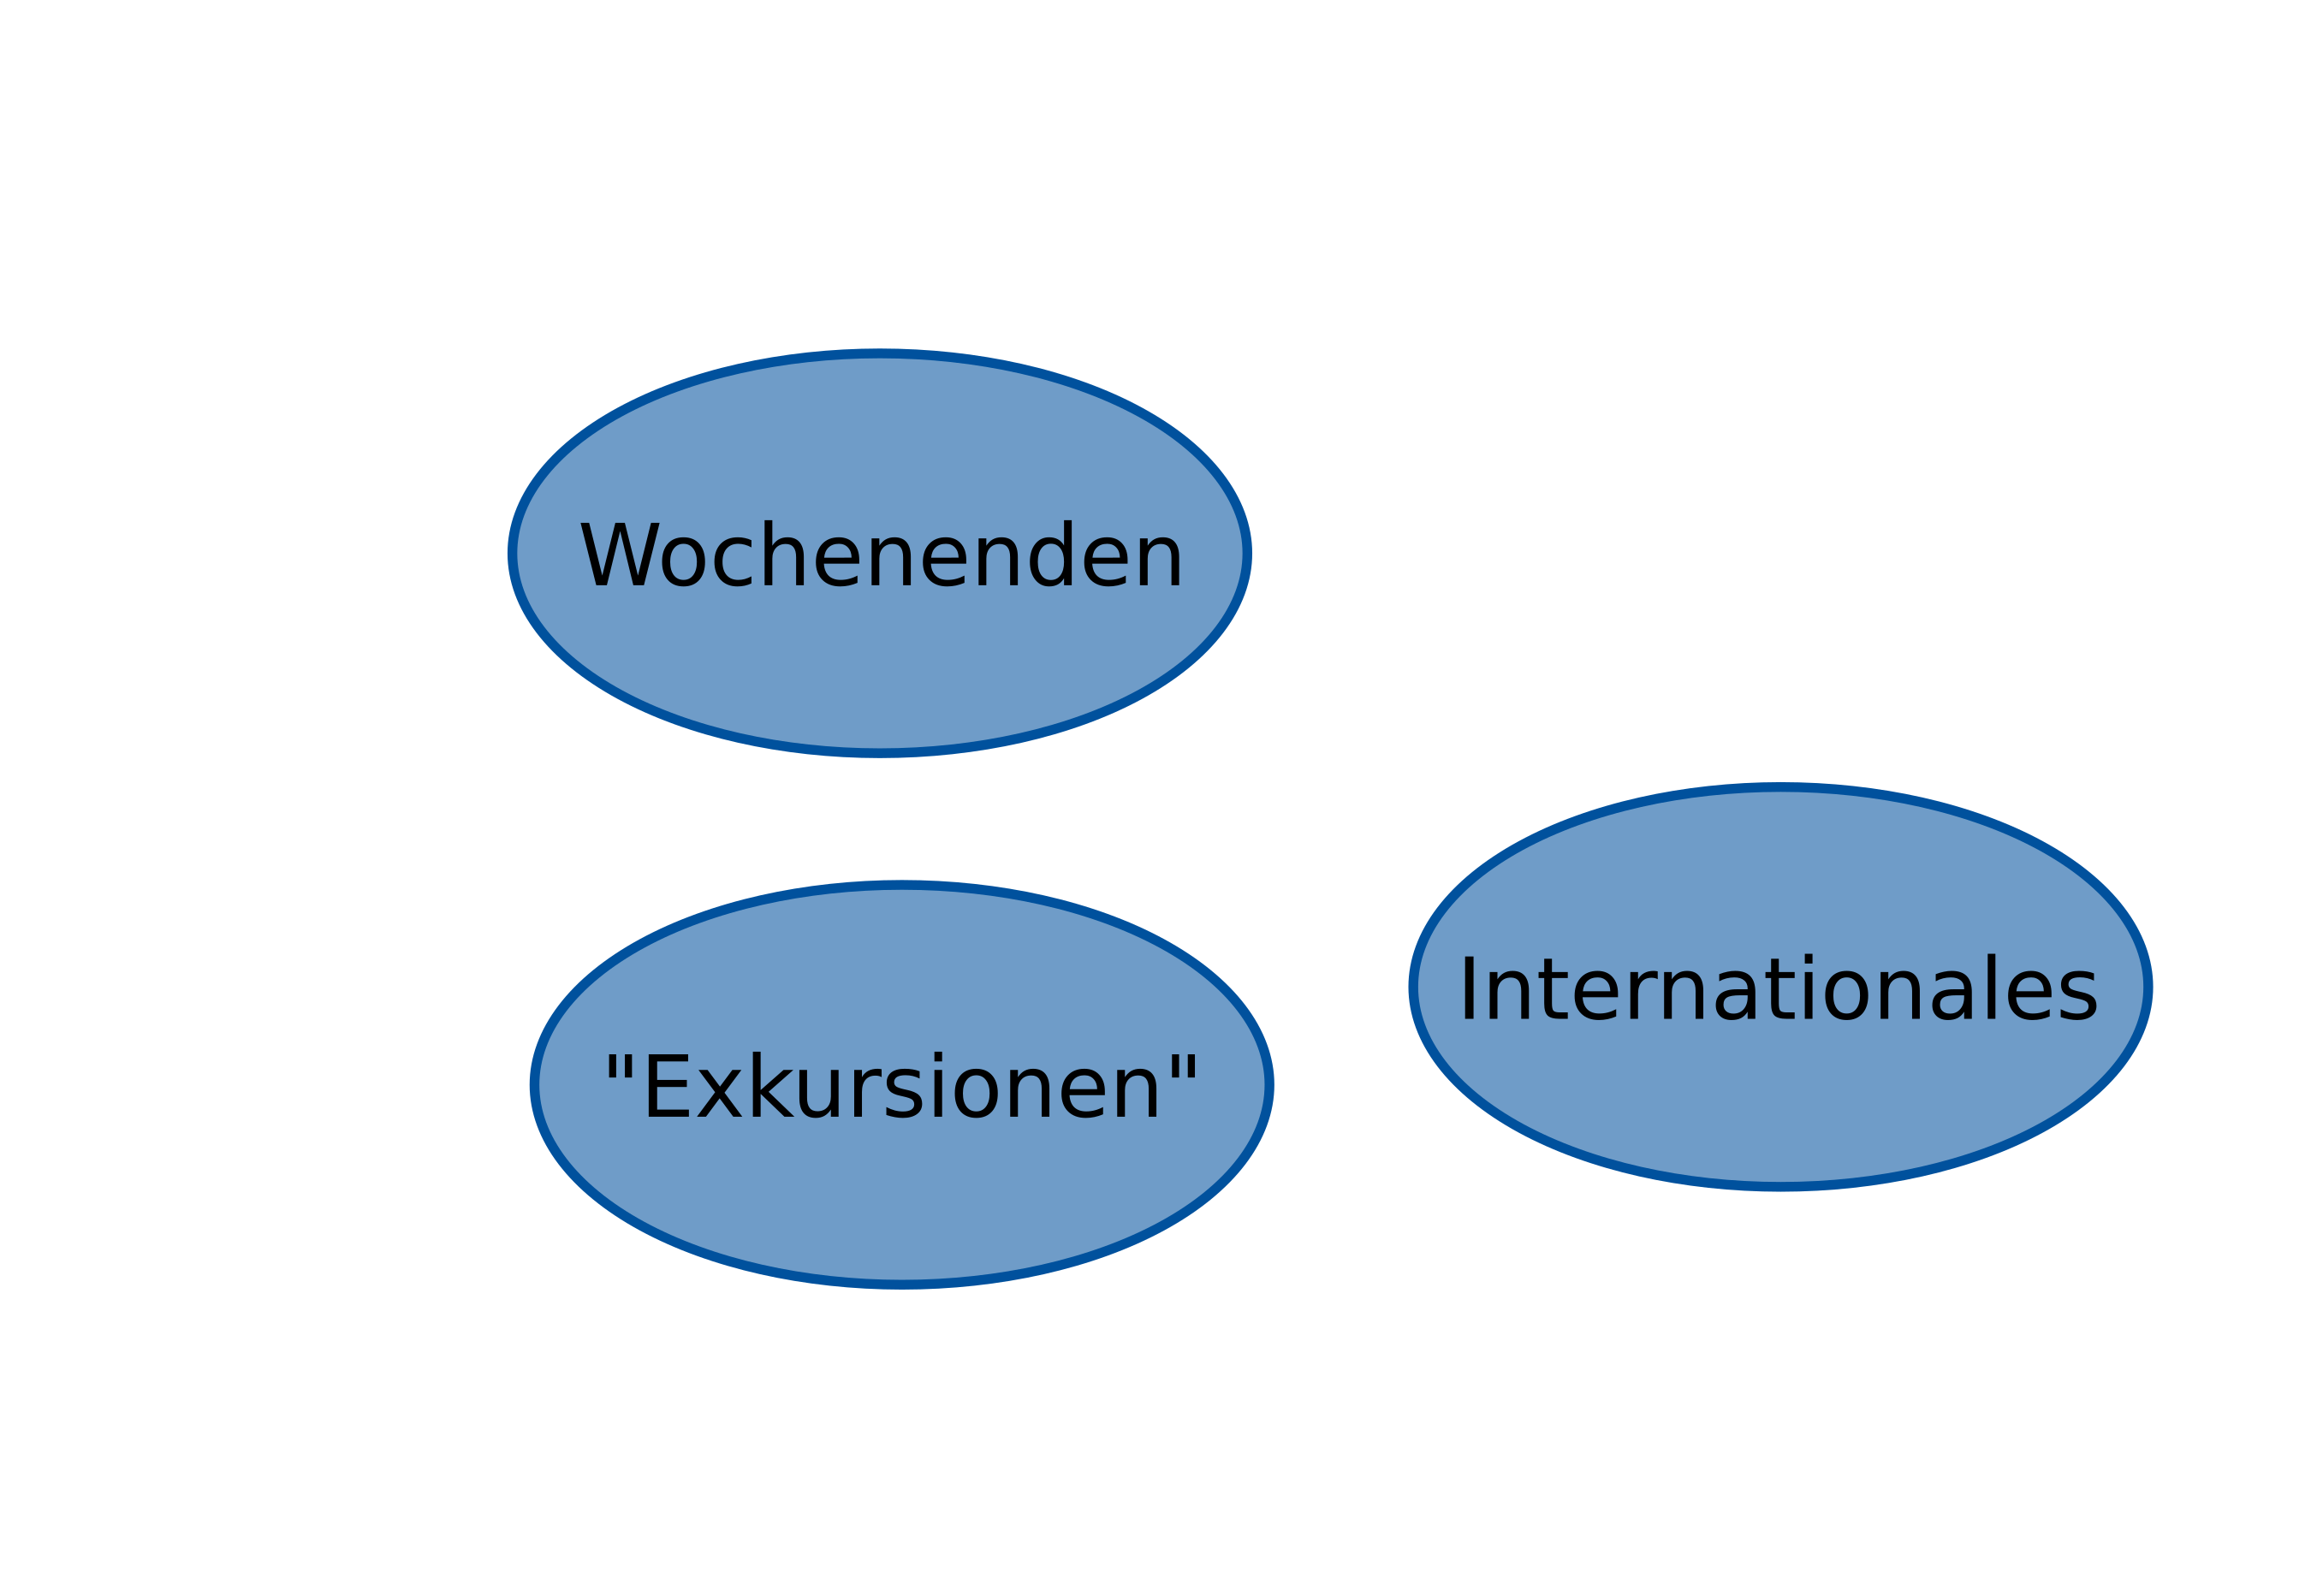
\includegraphics[width=0.80\textwidth]{figure/brainstormBundesweit_empty}
  \end{figure}
  \end{frame}

\begin{frame}{Gehirnsturm II}
\begin{figure}
 \centering
 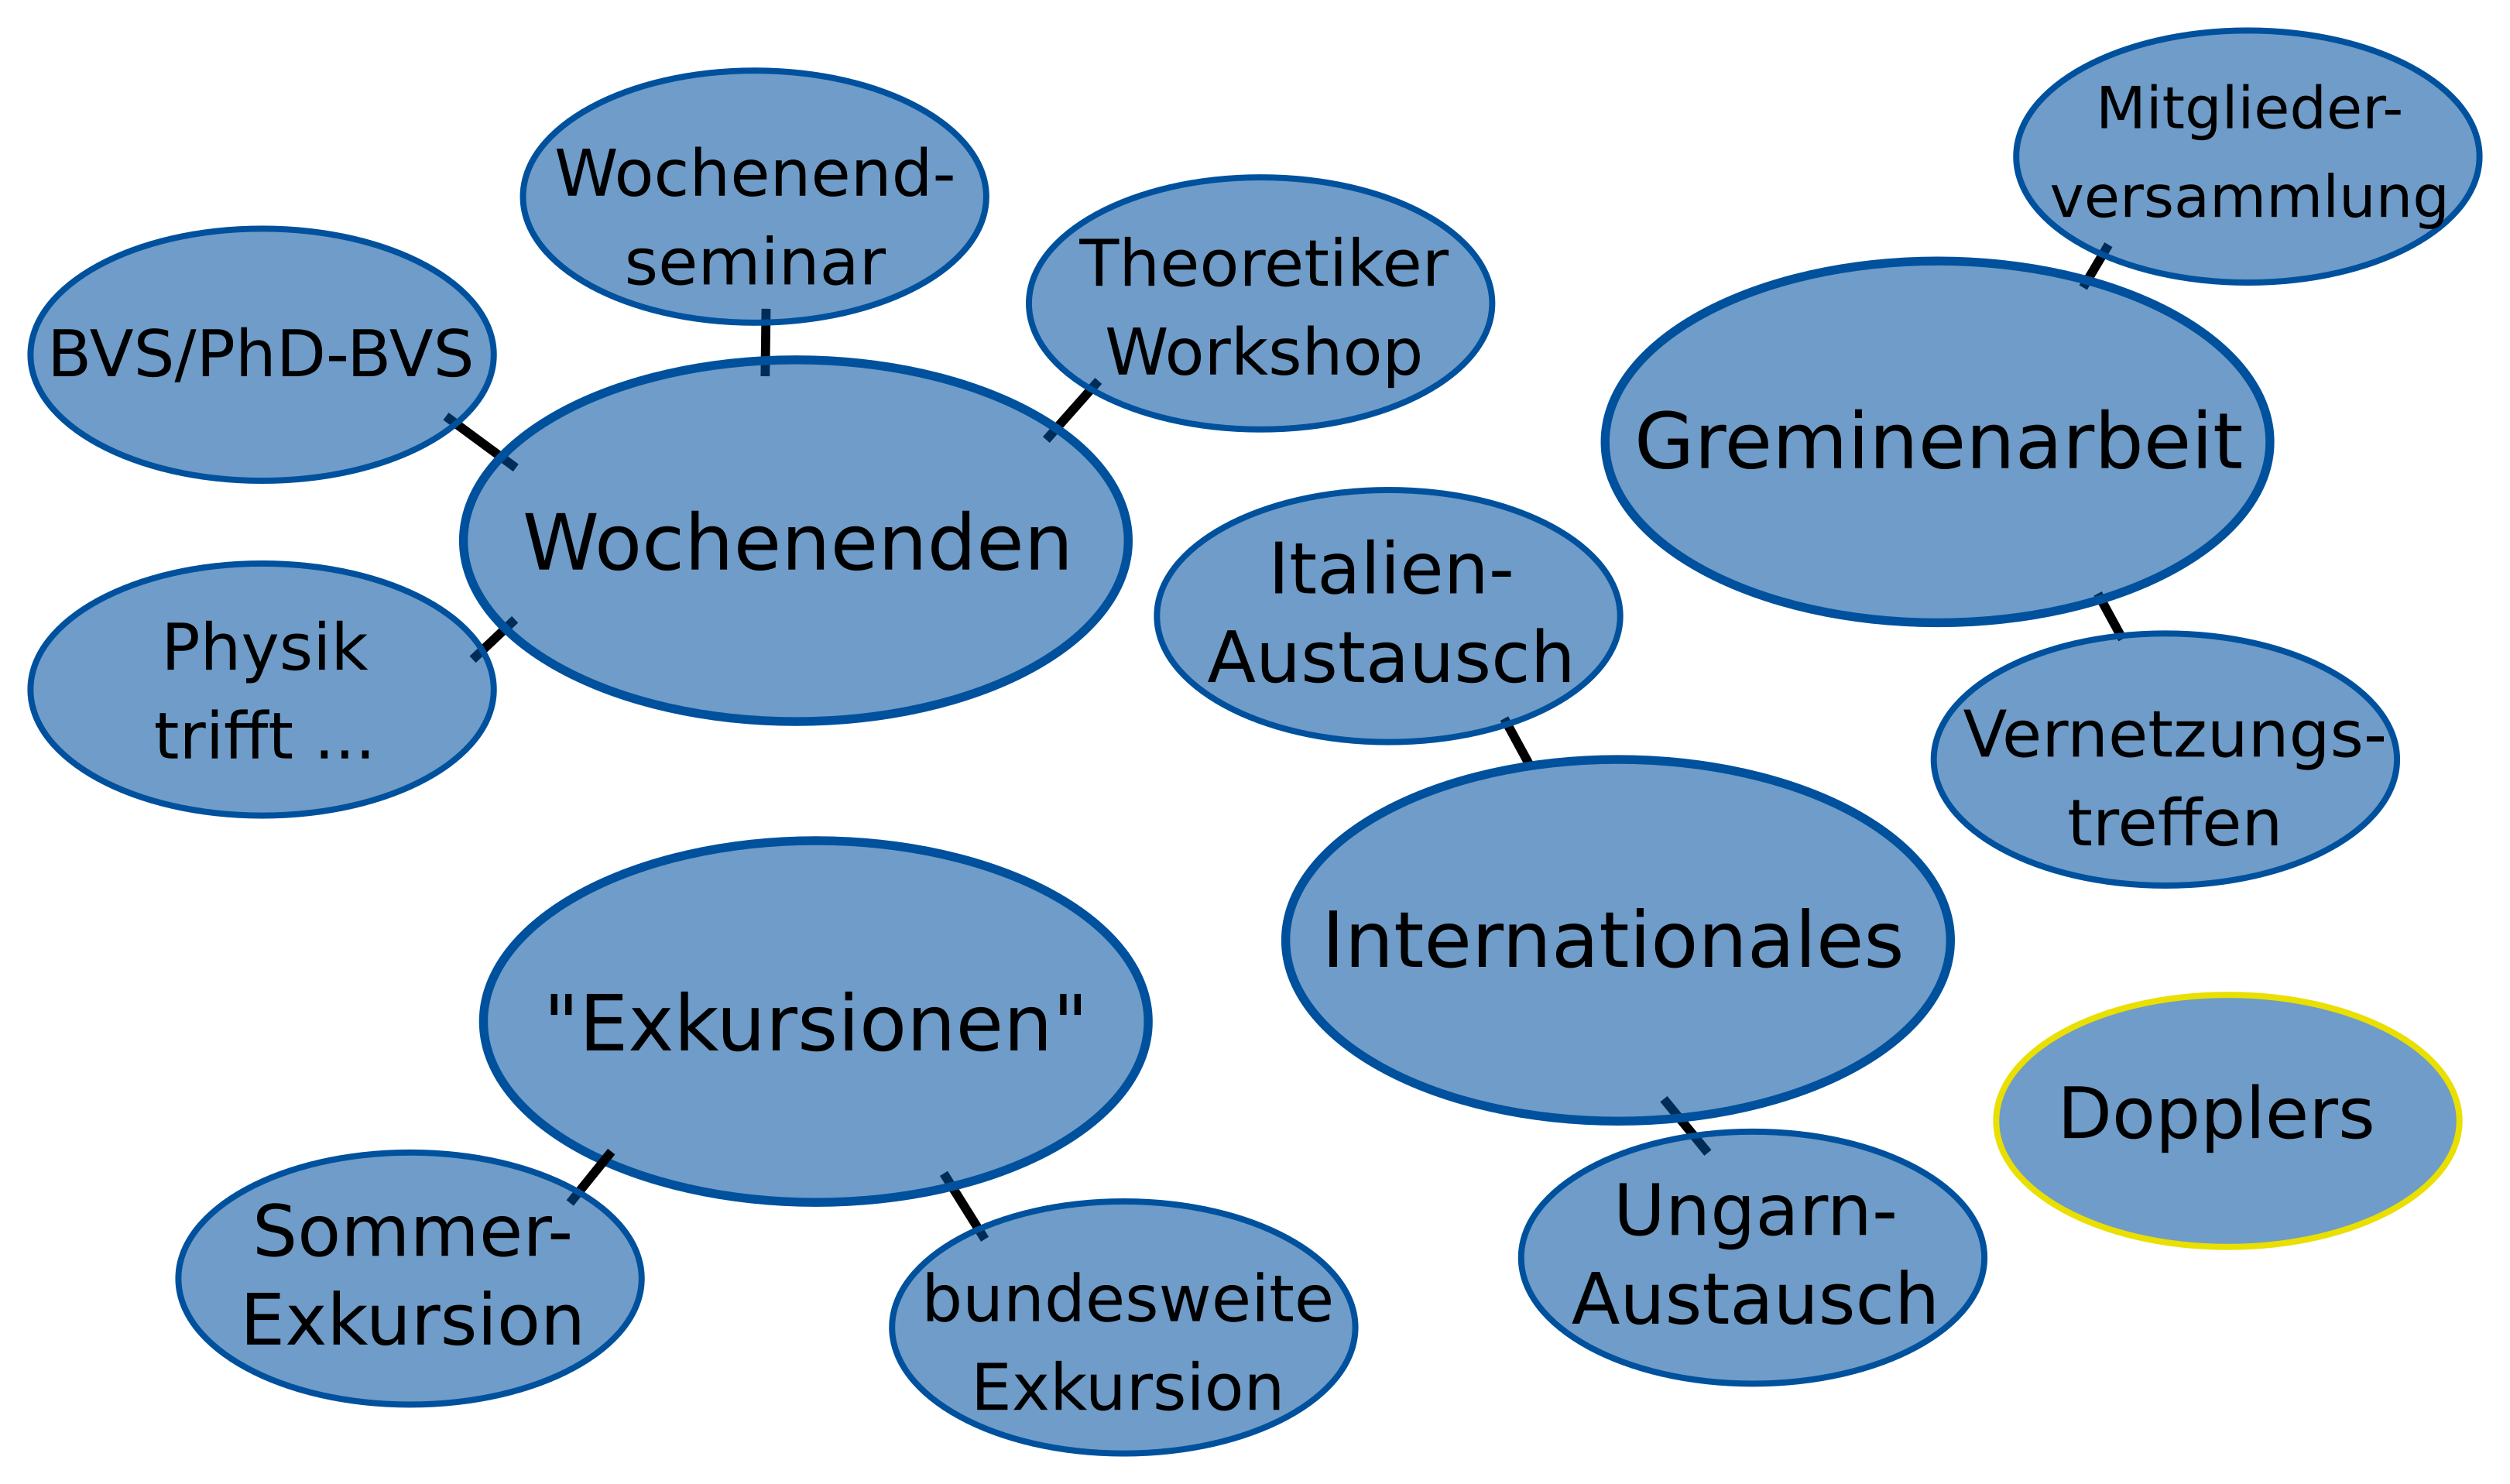
\includegraphics[width=0.80\textwidth]{figure/brainstormBundesweit_full}
\end{figure}
\end{frame}

\begin{frame}{Gremienarbeit}
  \begin{minipage}[0.3\textwidth]
    \begin{figure}
      \centering
      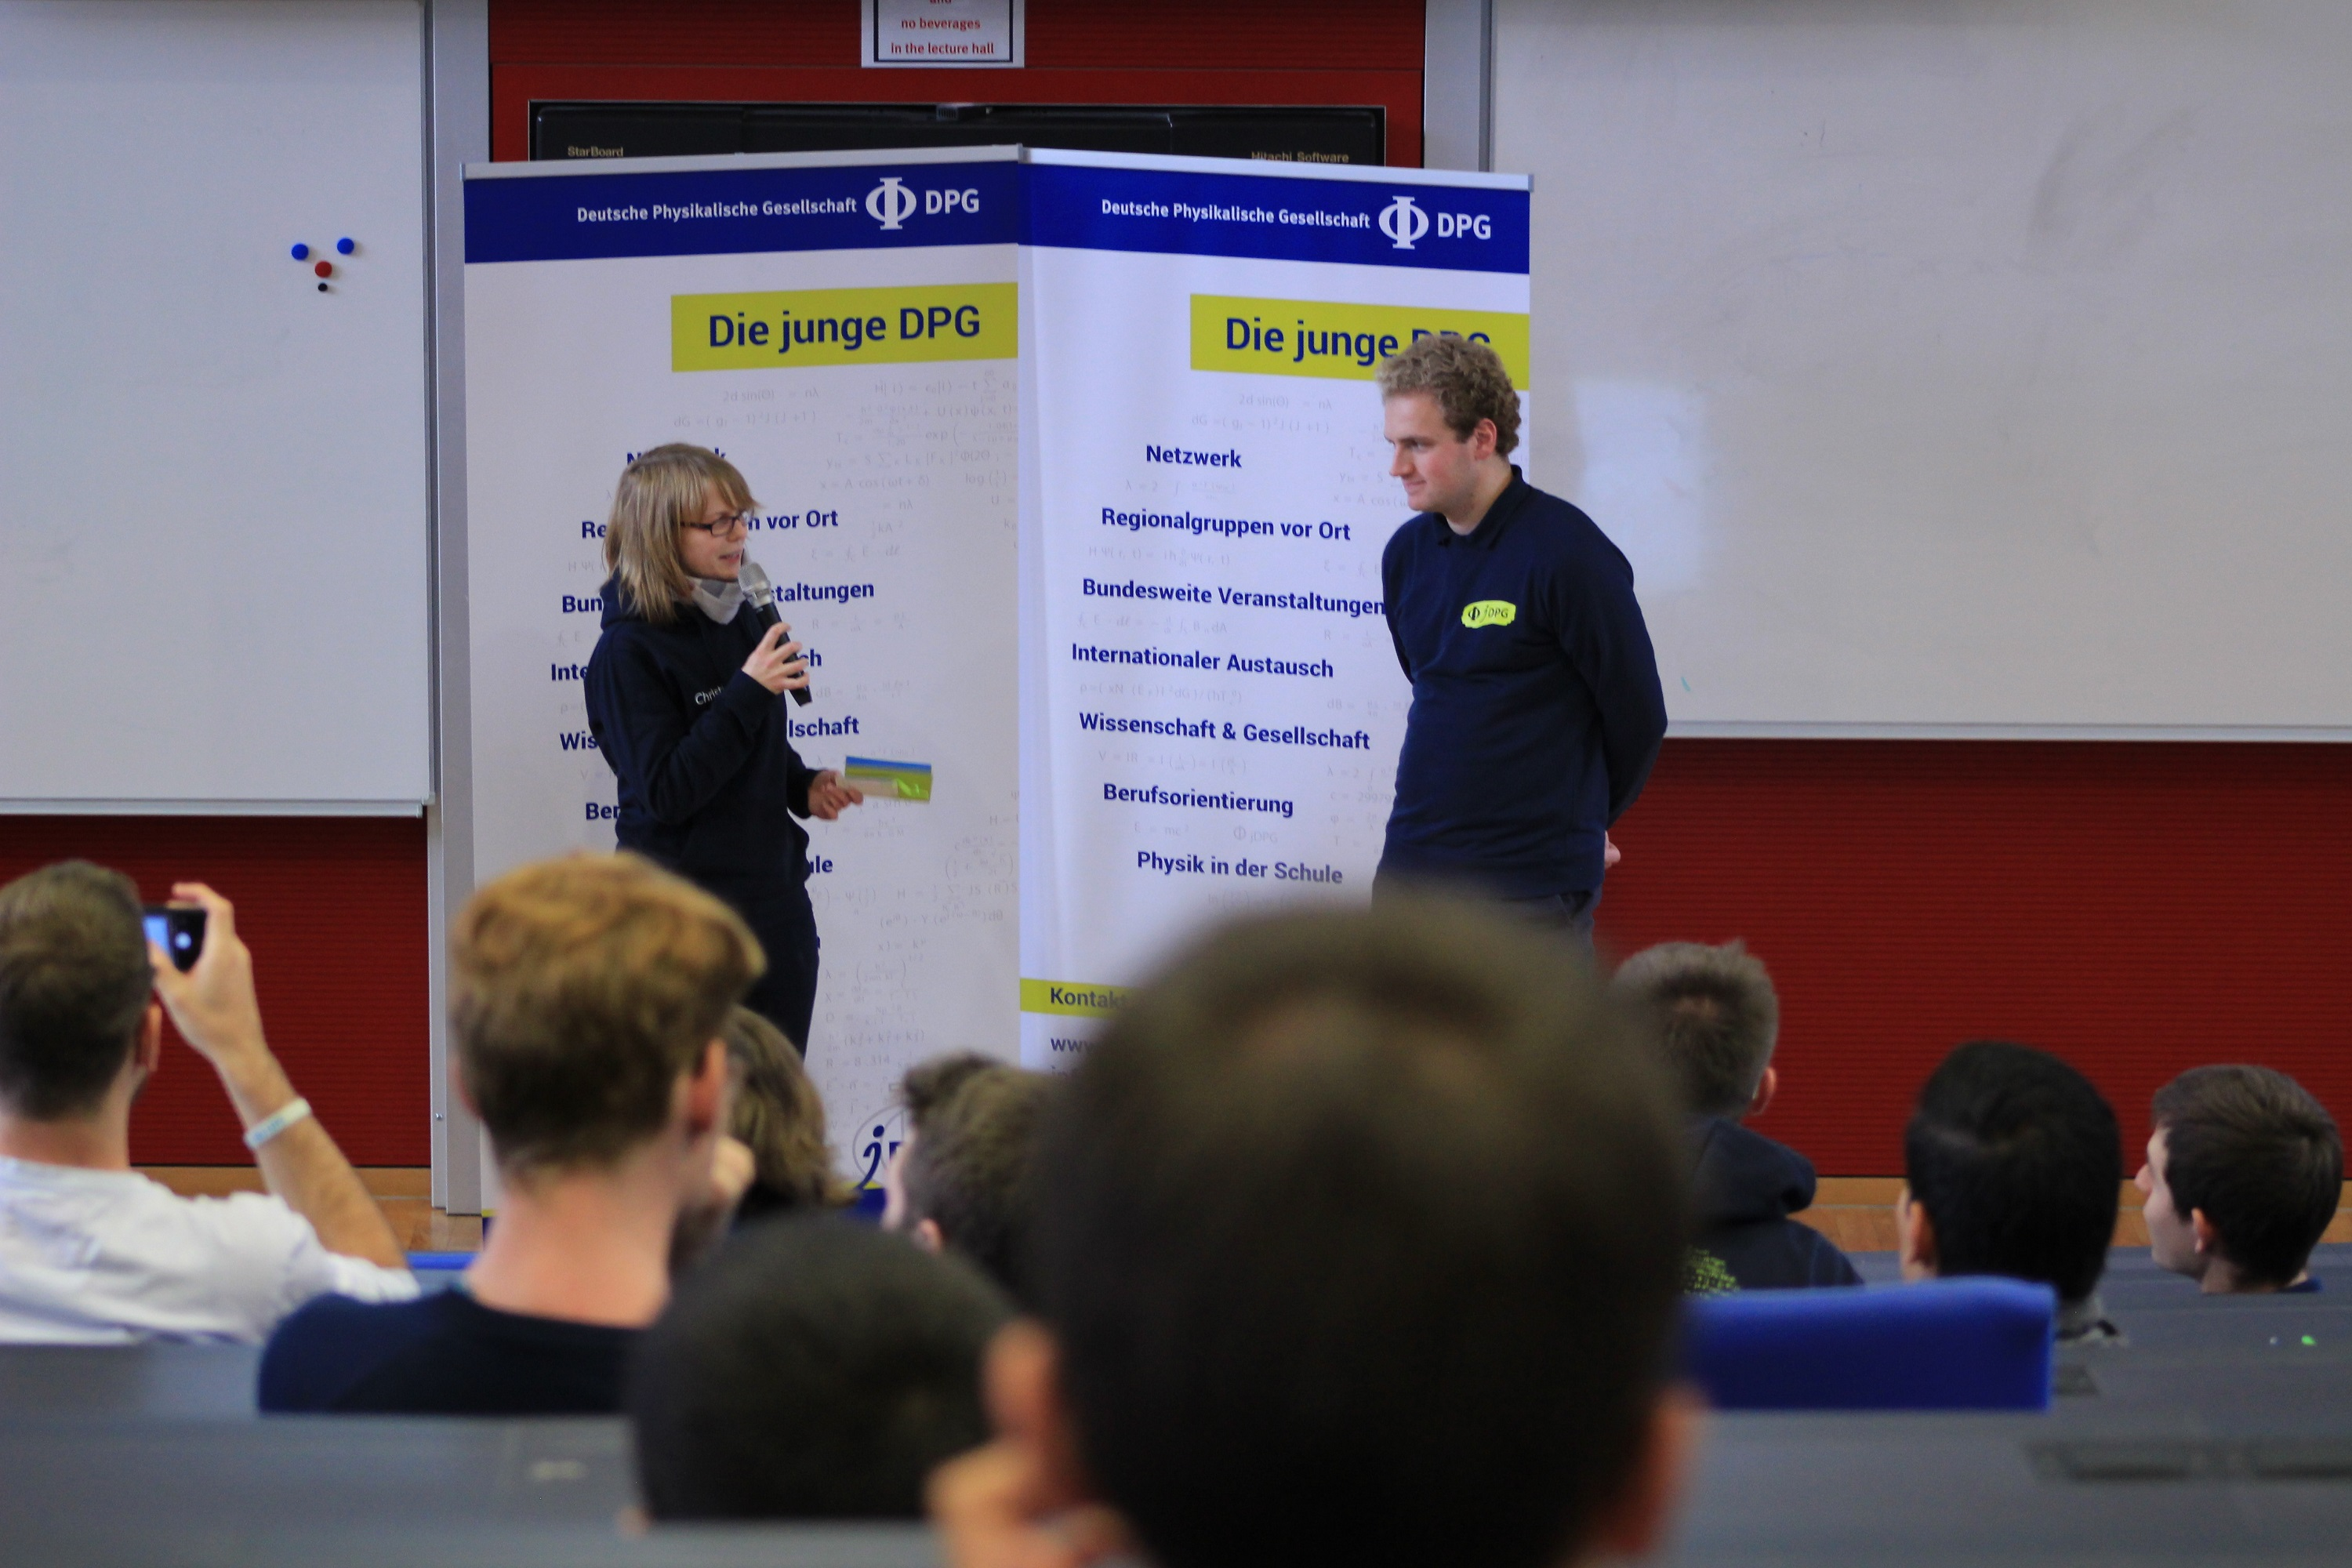
\includegraphics[width=0.99\textwidth]{figure/MV_2018_badHonnef_christina_mathias}
     \end{figure}
  \end{minipage}%
  \begin{minipage}[0.4\textwidth]
    \begin{itemize}
      \item Mitgliederversammlung\\
      jDPG Wochenende
    \end{itemize}
    Workshops, Wahlen, Entlastung Vorstand
  \end{minipage}
  \begin{minipage}[0.3\textwidth]
    \begin{figure}
      \centering
      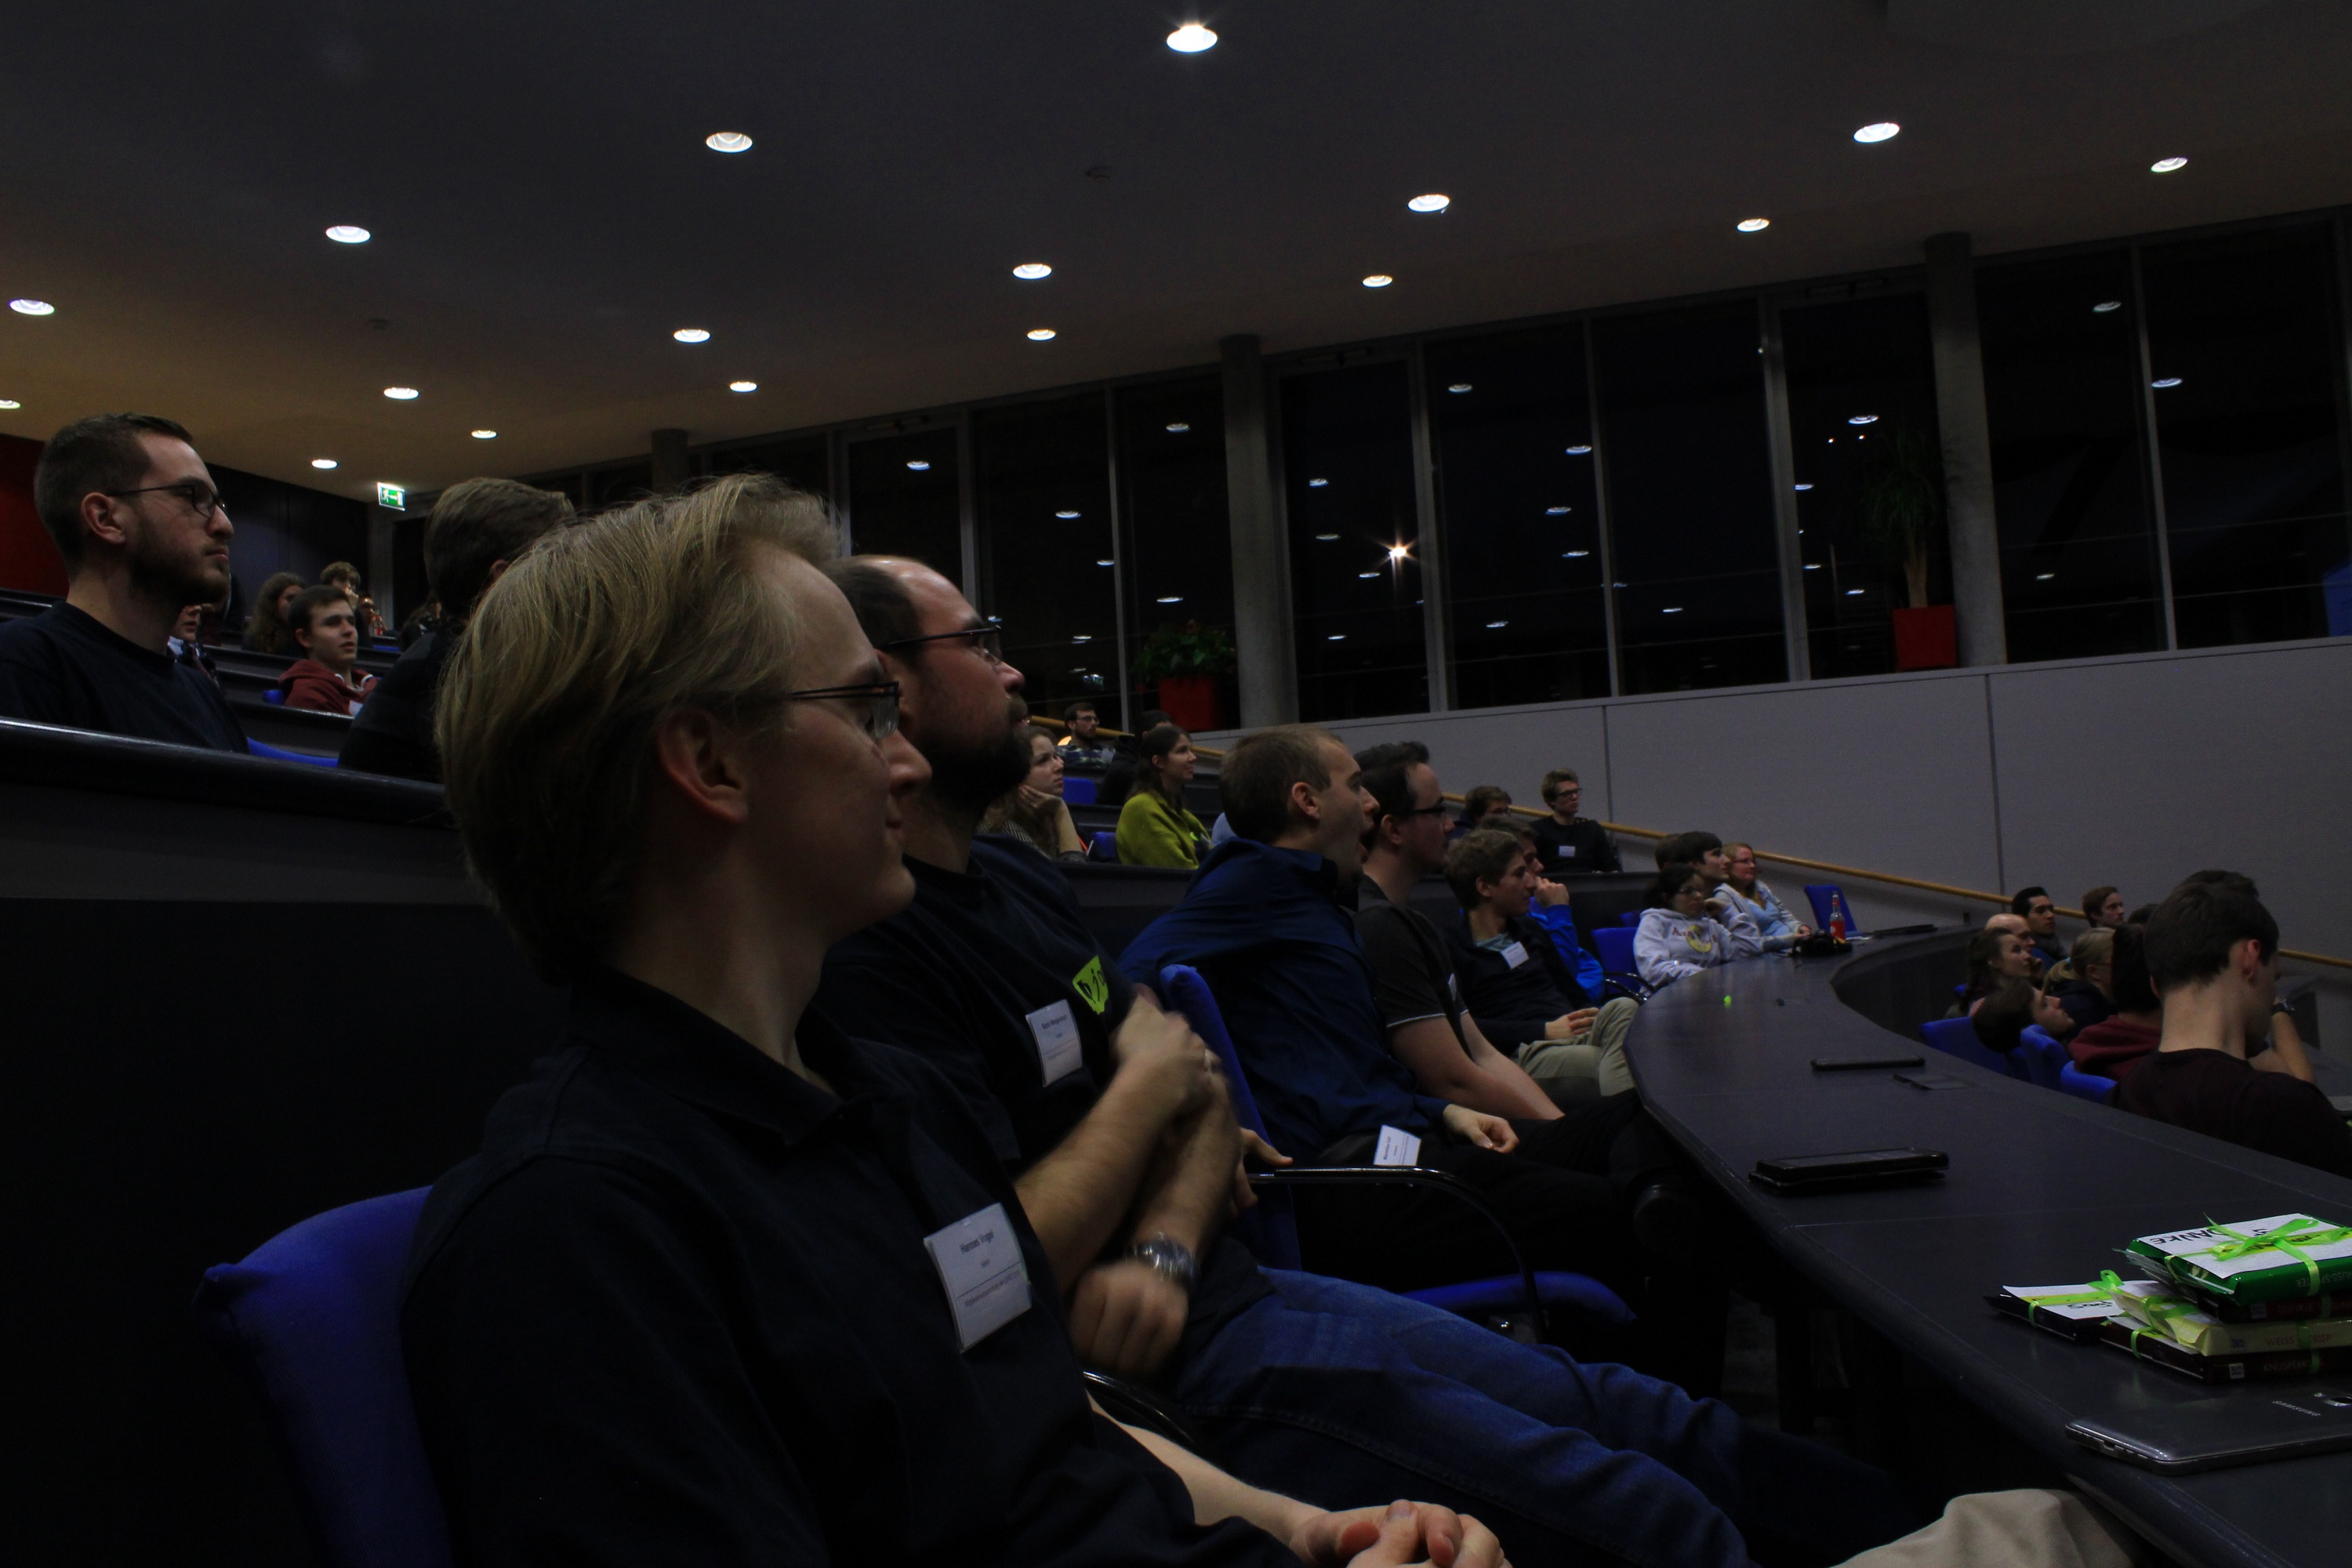
\includegraphics[width=0.99\textwidth]{figure/MV_2018_badHonnef_publikum}
     \end{figure}
  \end{minipage}

  \begin{minipage}[0.4\textwidth]
    \begin{itemize}
      \item Vernetzungstreffen
    \end{itemize}
    Austausch zwischen Regionalgruppen und Vertiefung jDPG-Wissen
  \end{minipage}%
  \begin{minipage}[0.6\textwidth]
    \begin{figure}
      \centering
      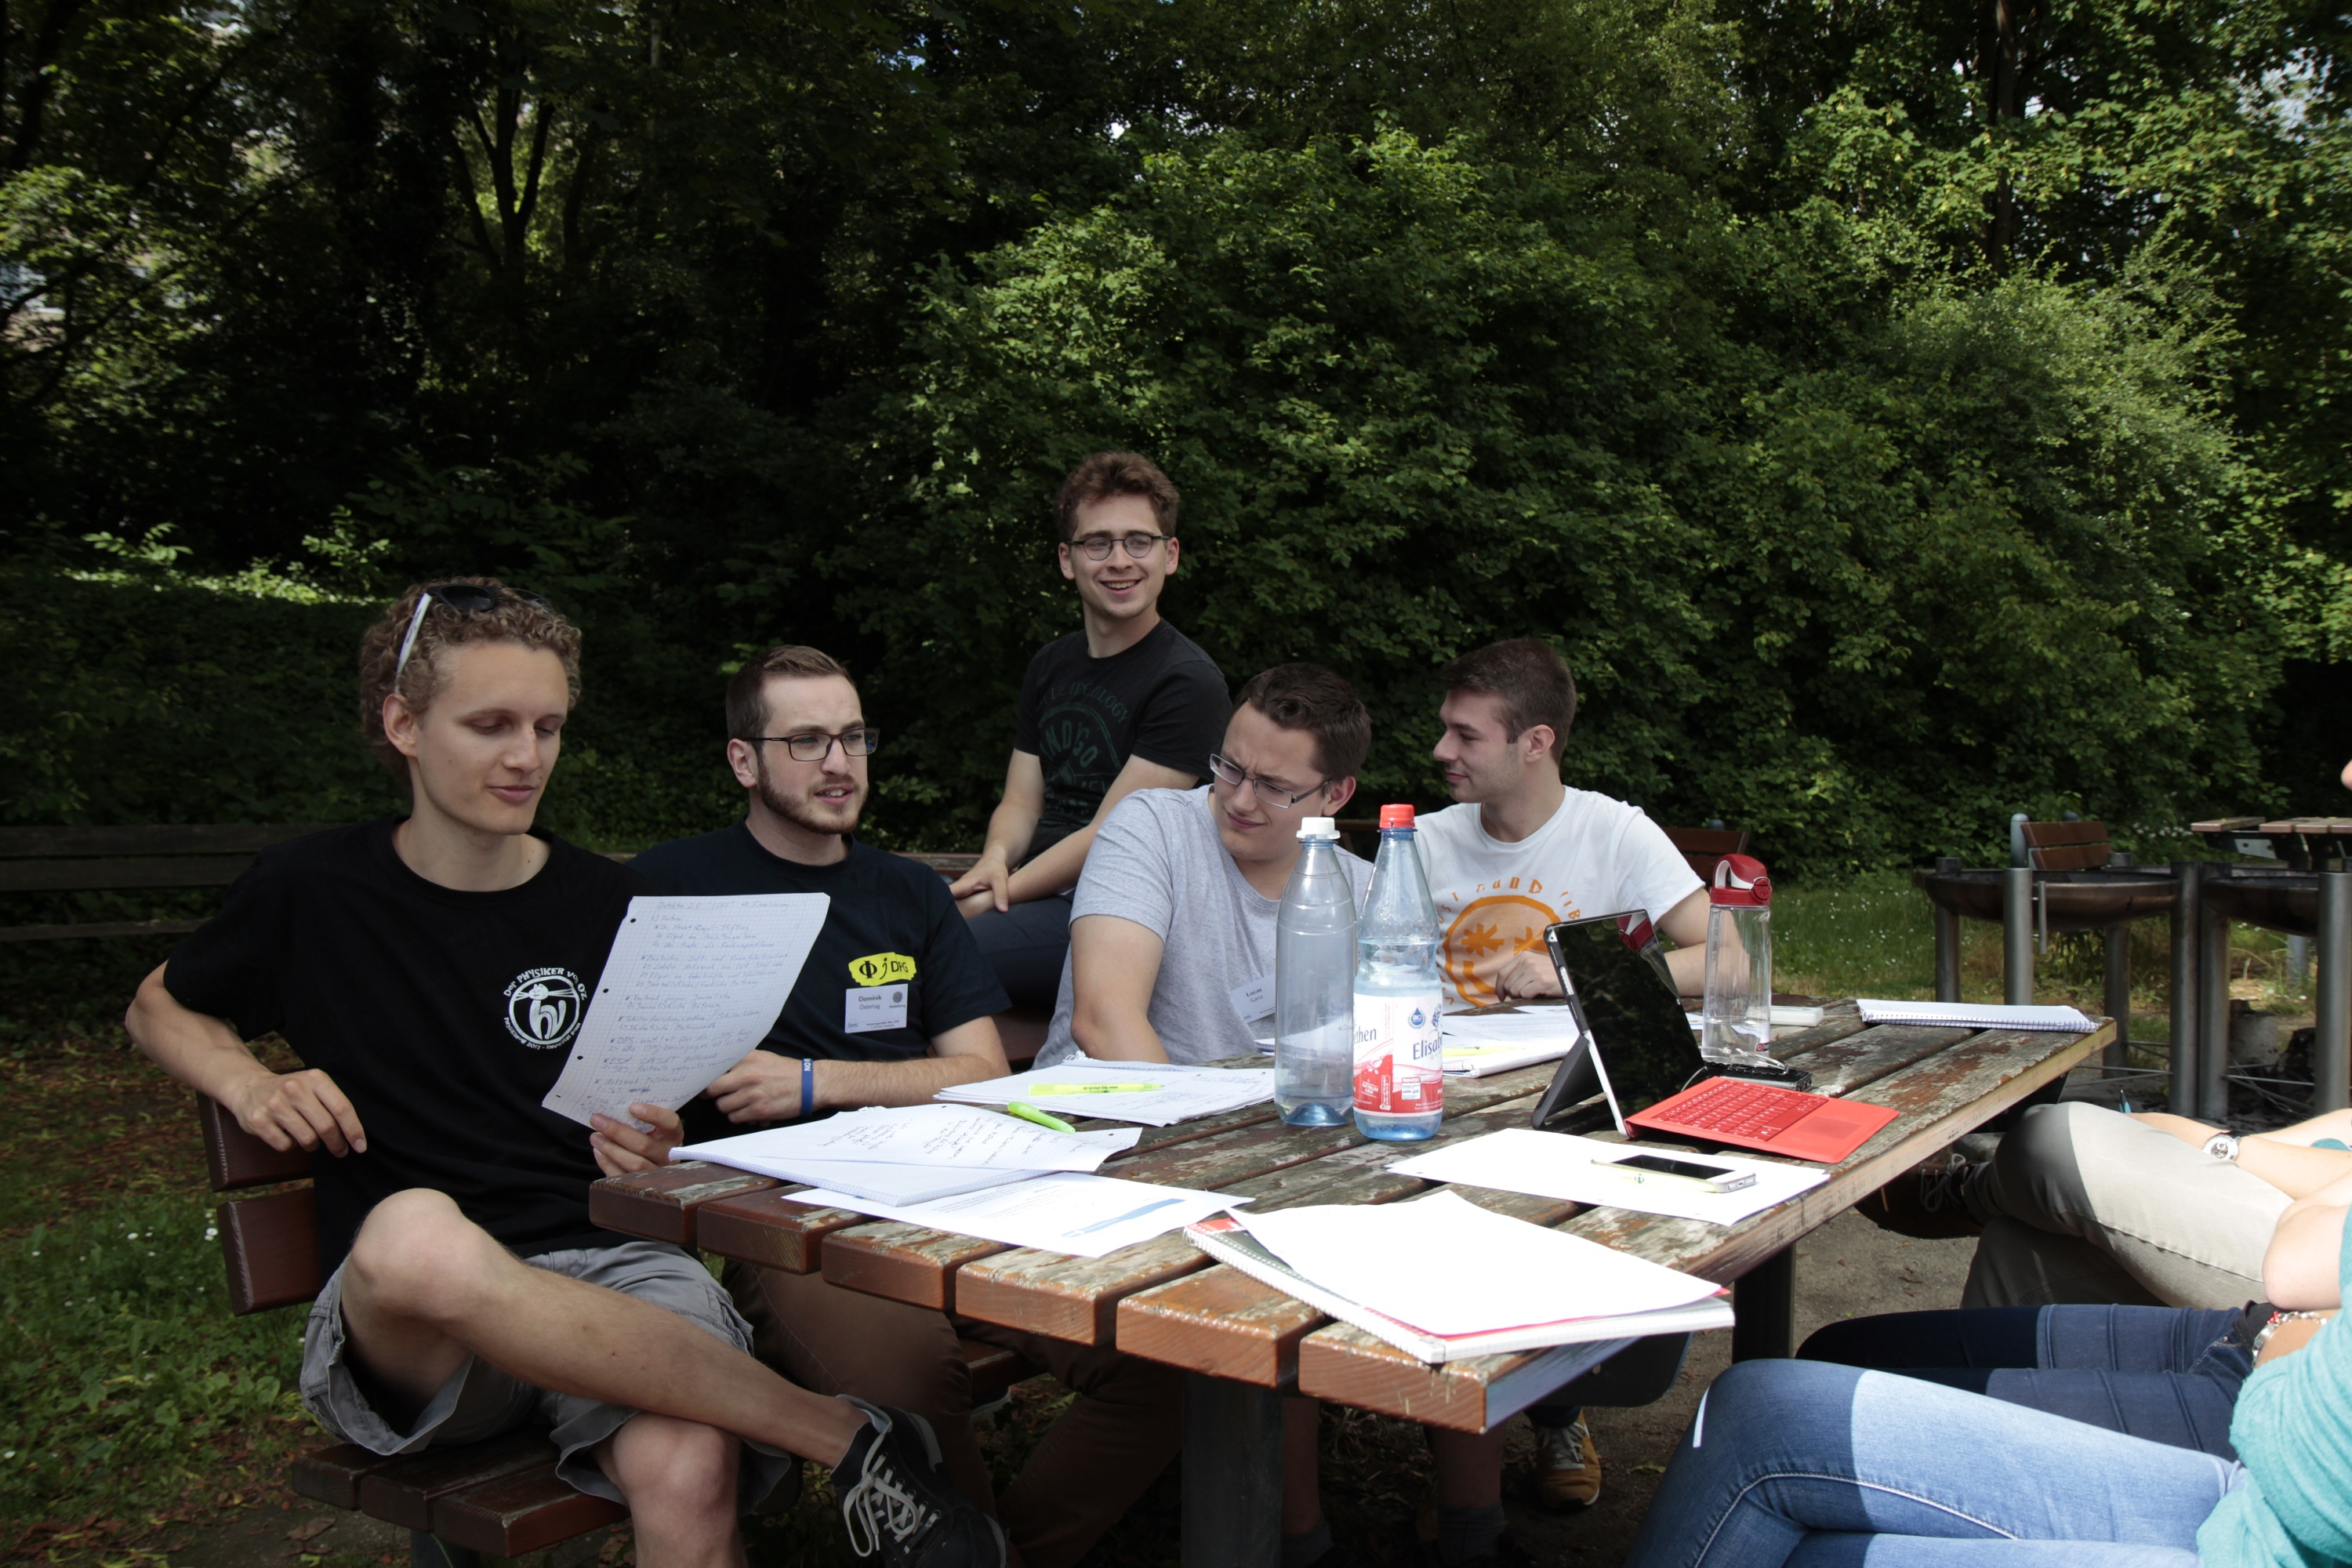
\includegraphics[width=0.49\textwidth]{figure/VT-West-2018_Austausch}\hfill
      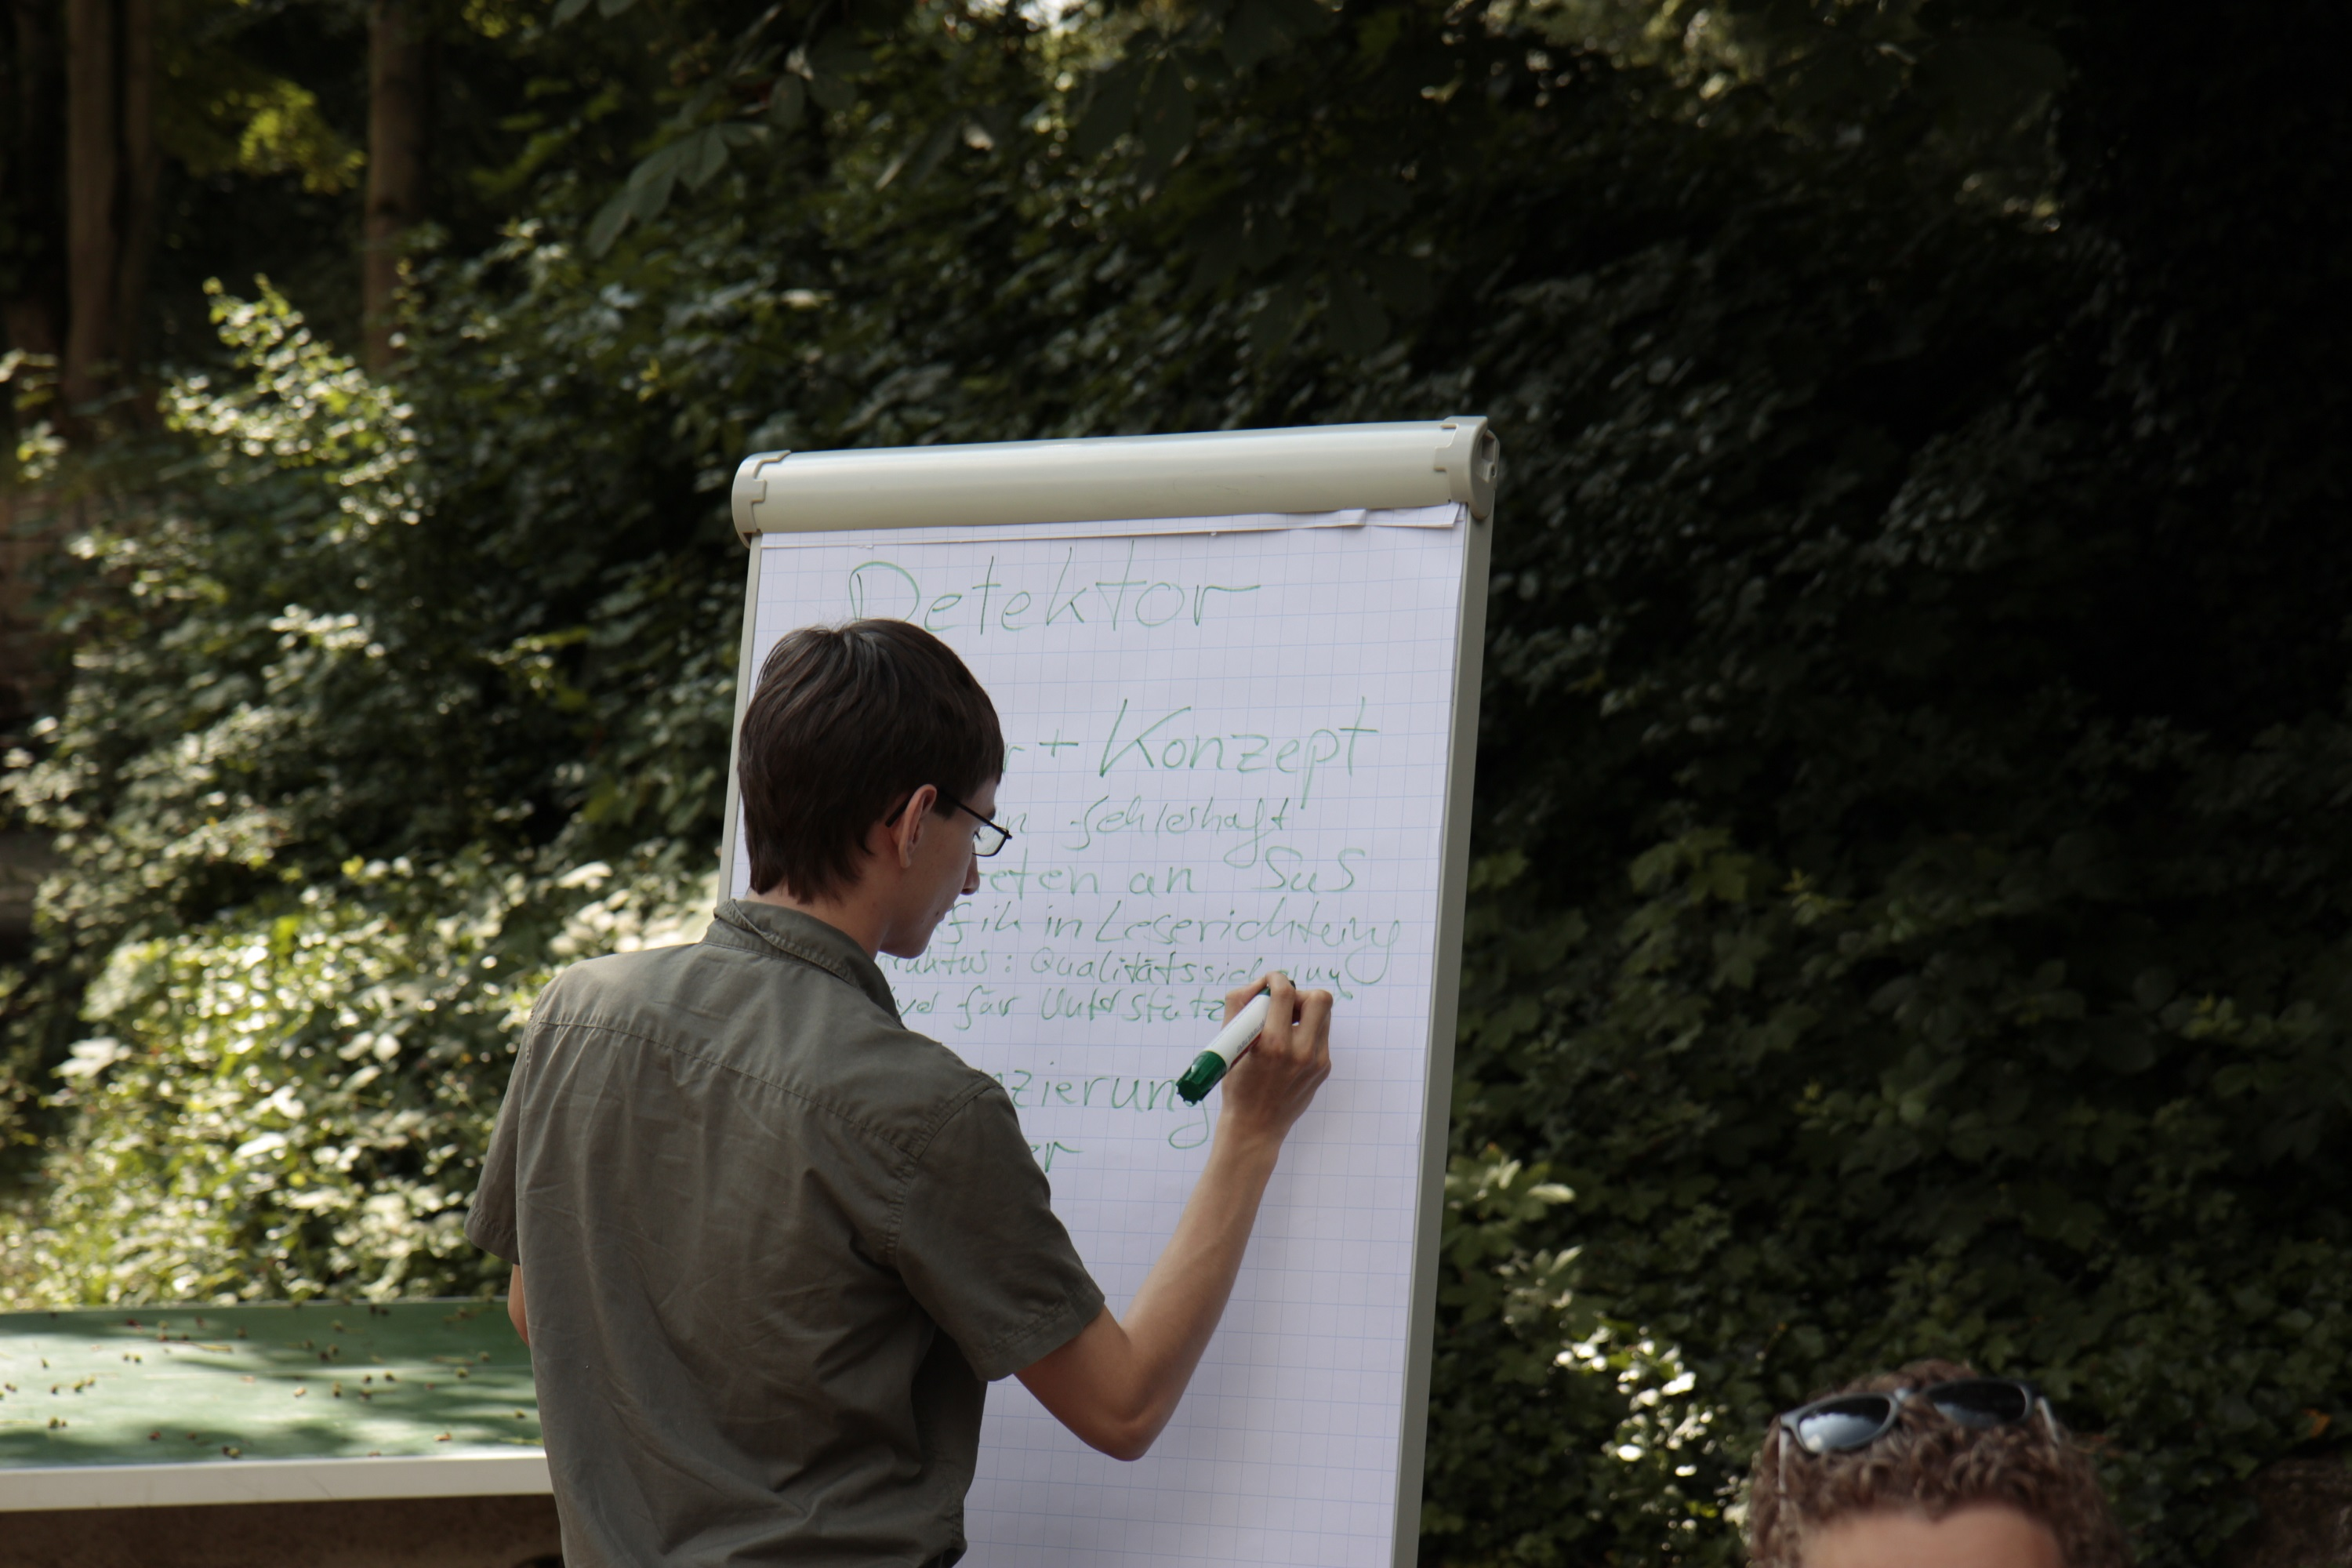
\includegraphics[width=0.49\textwidth]{figure/VT-West-2018_wissen}\\
      \begin{center}
        Vernetzungstreffen West 2018
      \end{center}
     \end{figure}
  \end{minipage}
\end{frame}

\begin{frame}{intensive Wochenenden}
  \begin{minipage}[0.4\textwidth]
    \begin{itemize}
      \item Theoretikerworkshop
      \item Wochenendseminar
      \item Umweltseminar
      \item Physik trifft ...
    \end{itemize}
    drei Tage, ein Thema
  \end{minipage}
  \begin{minipage}[0.6\textwidth]
    \begin{figure}
      \centering
      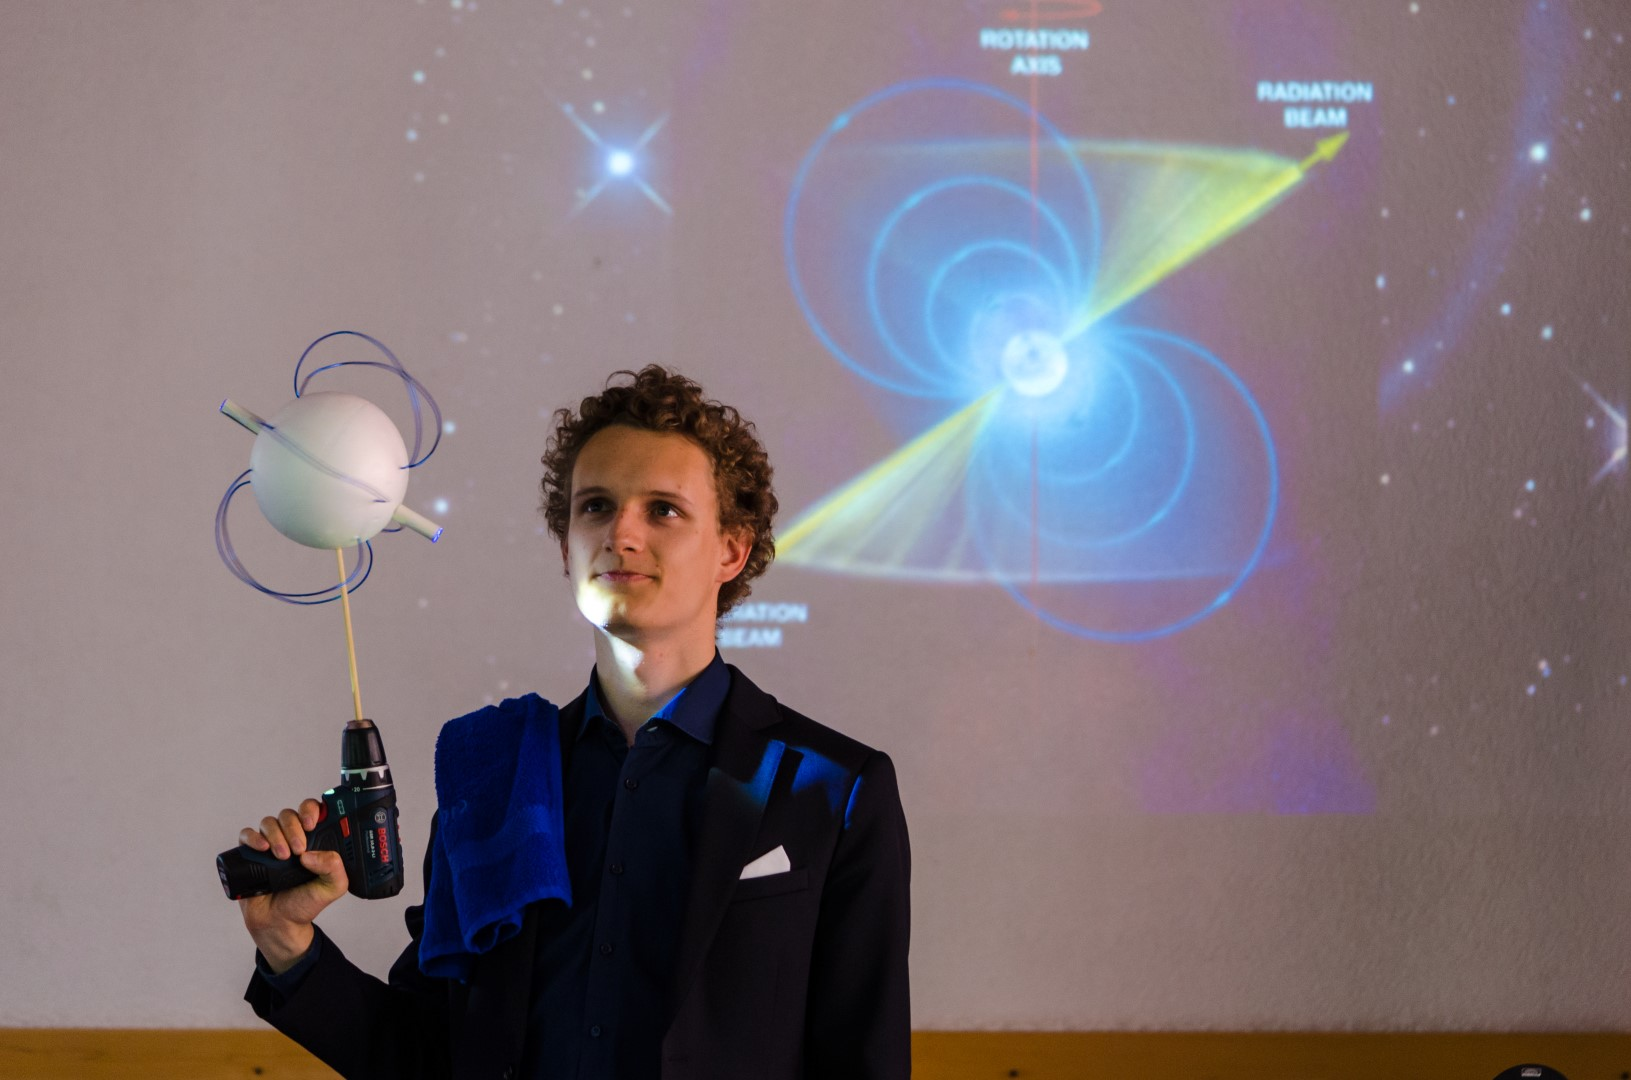
\includegraphics[width=0.49\textwidth]{figure/astrogastro_2017_david}\hfill
      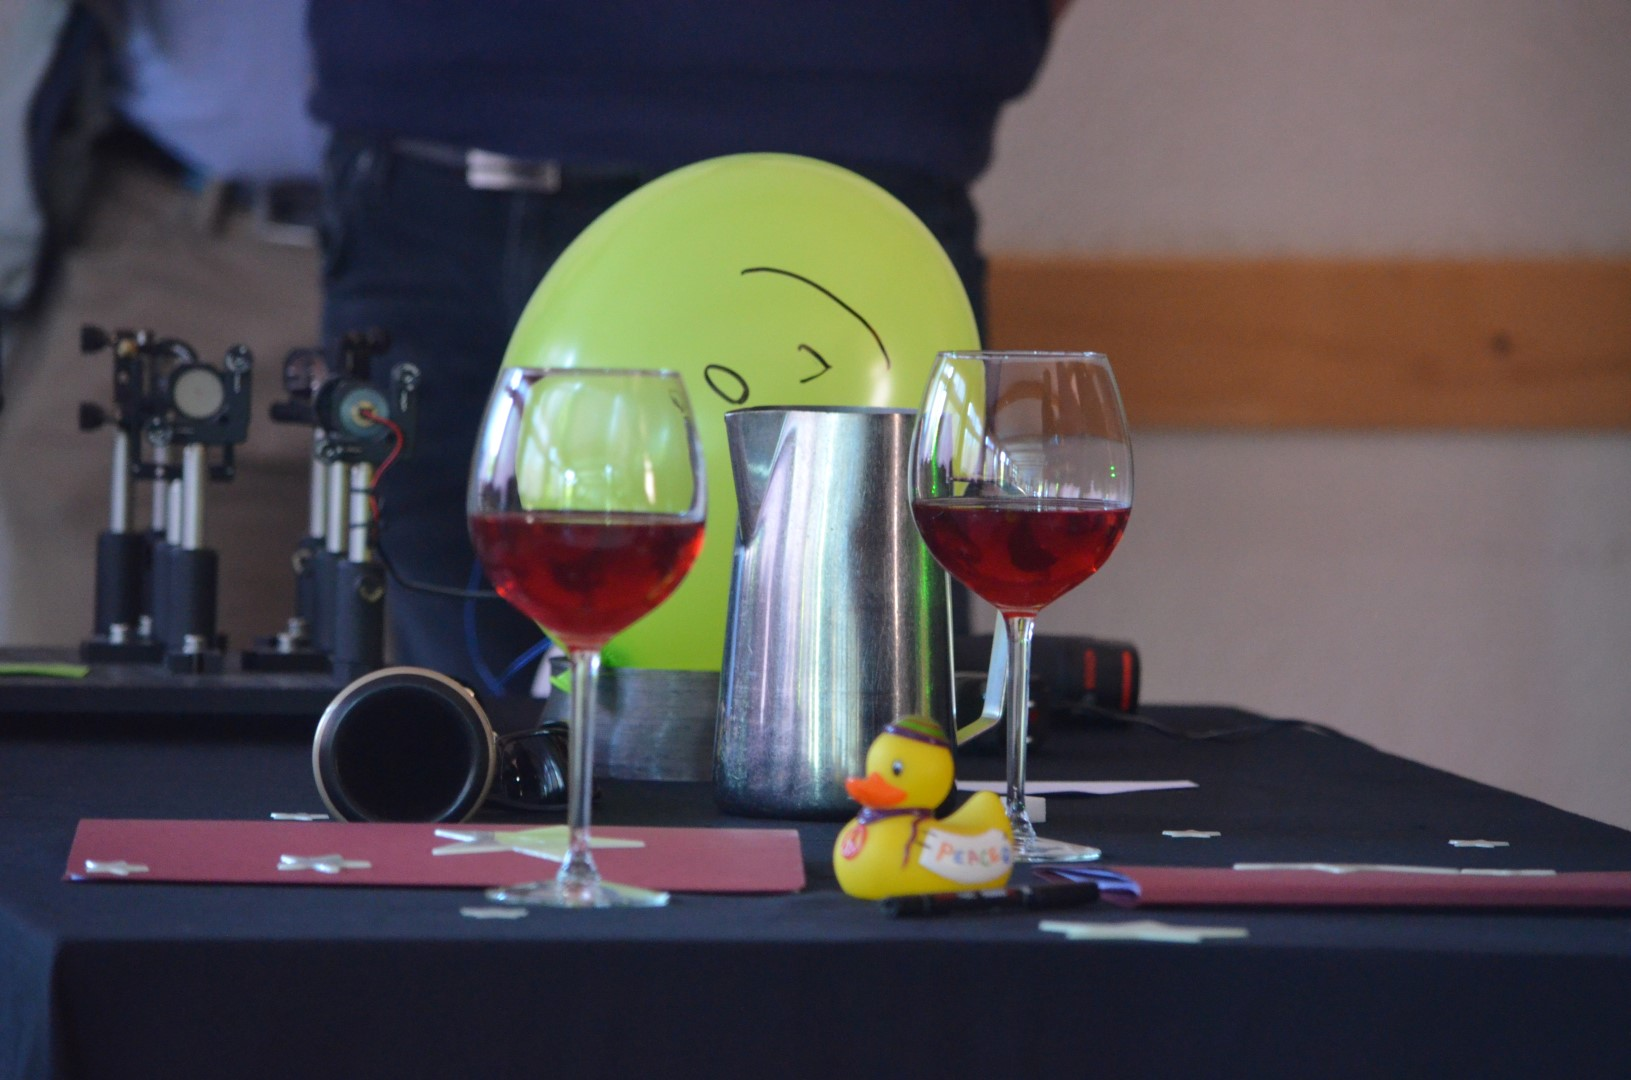
\includegraphics[width=0.49\textwidth]{figure/astrogastro_2017_wein}\\
      \begin{center}
        AstroGastro 2017 $\rightarrow$ Physik trifft Gastronomie
      \end{center}
     \end{figure}
  \end{minipage}
  
  \begin{minipage}[0.6\textwidth]
    \begin{figure}
      \centering
      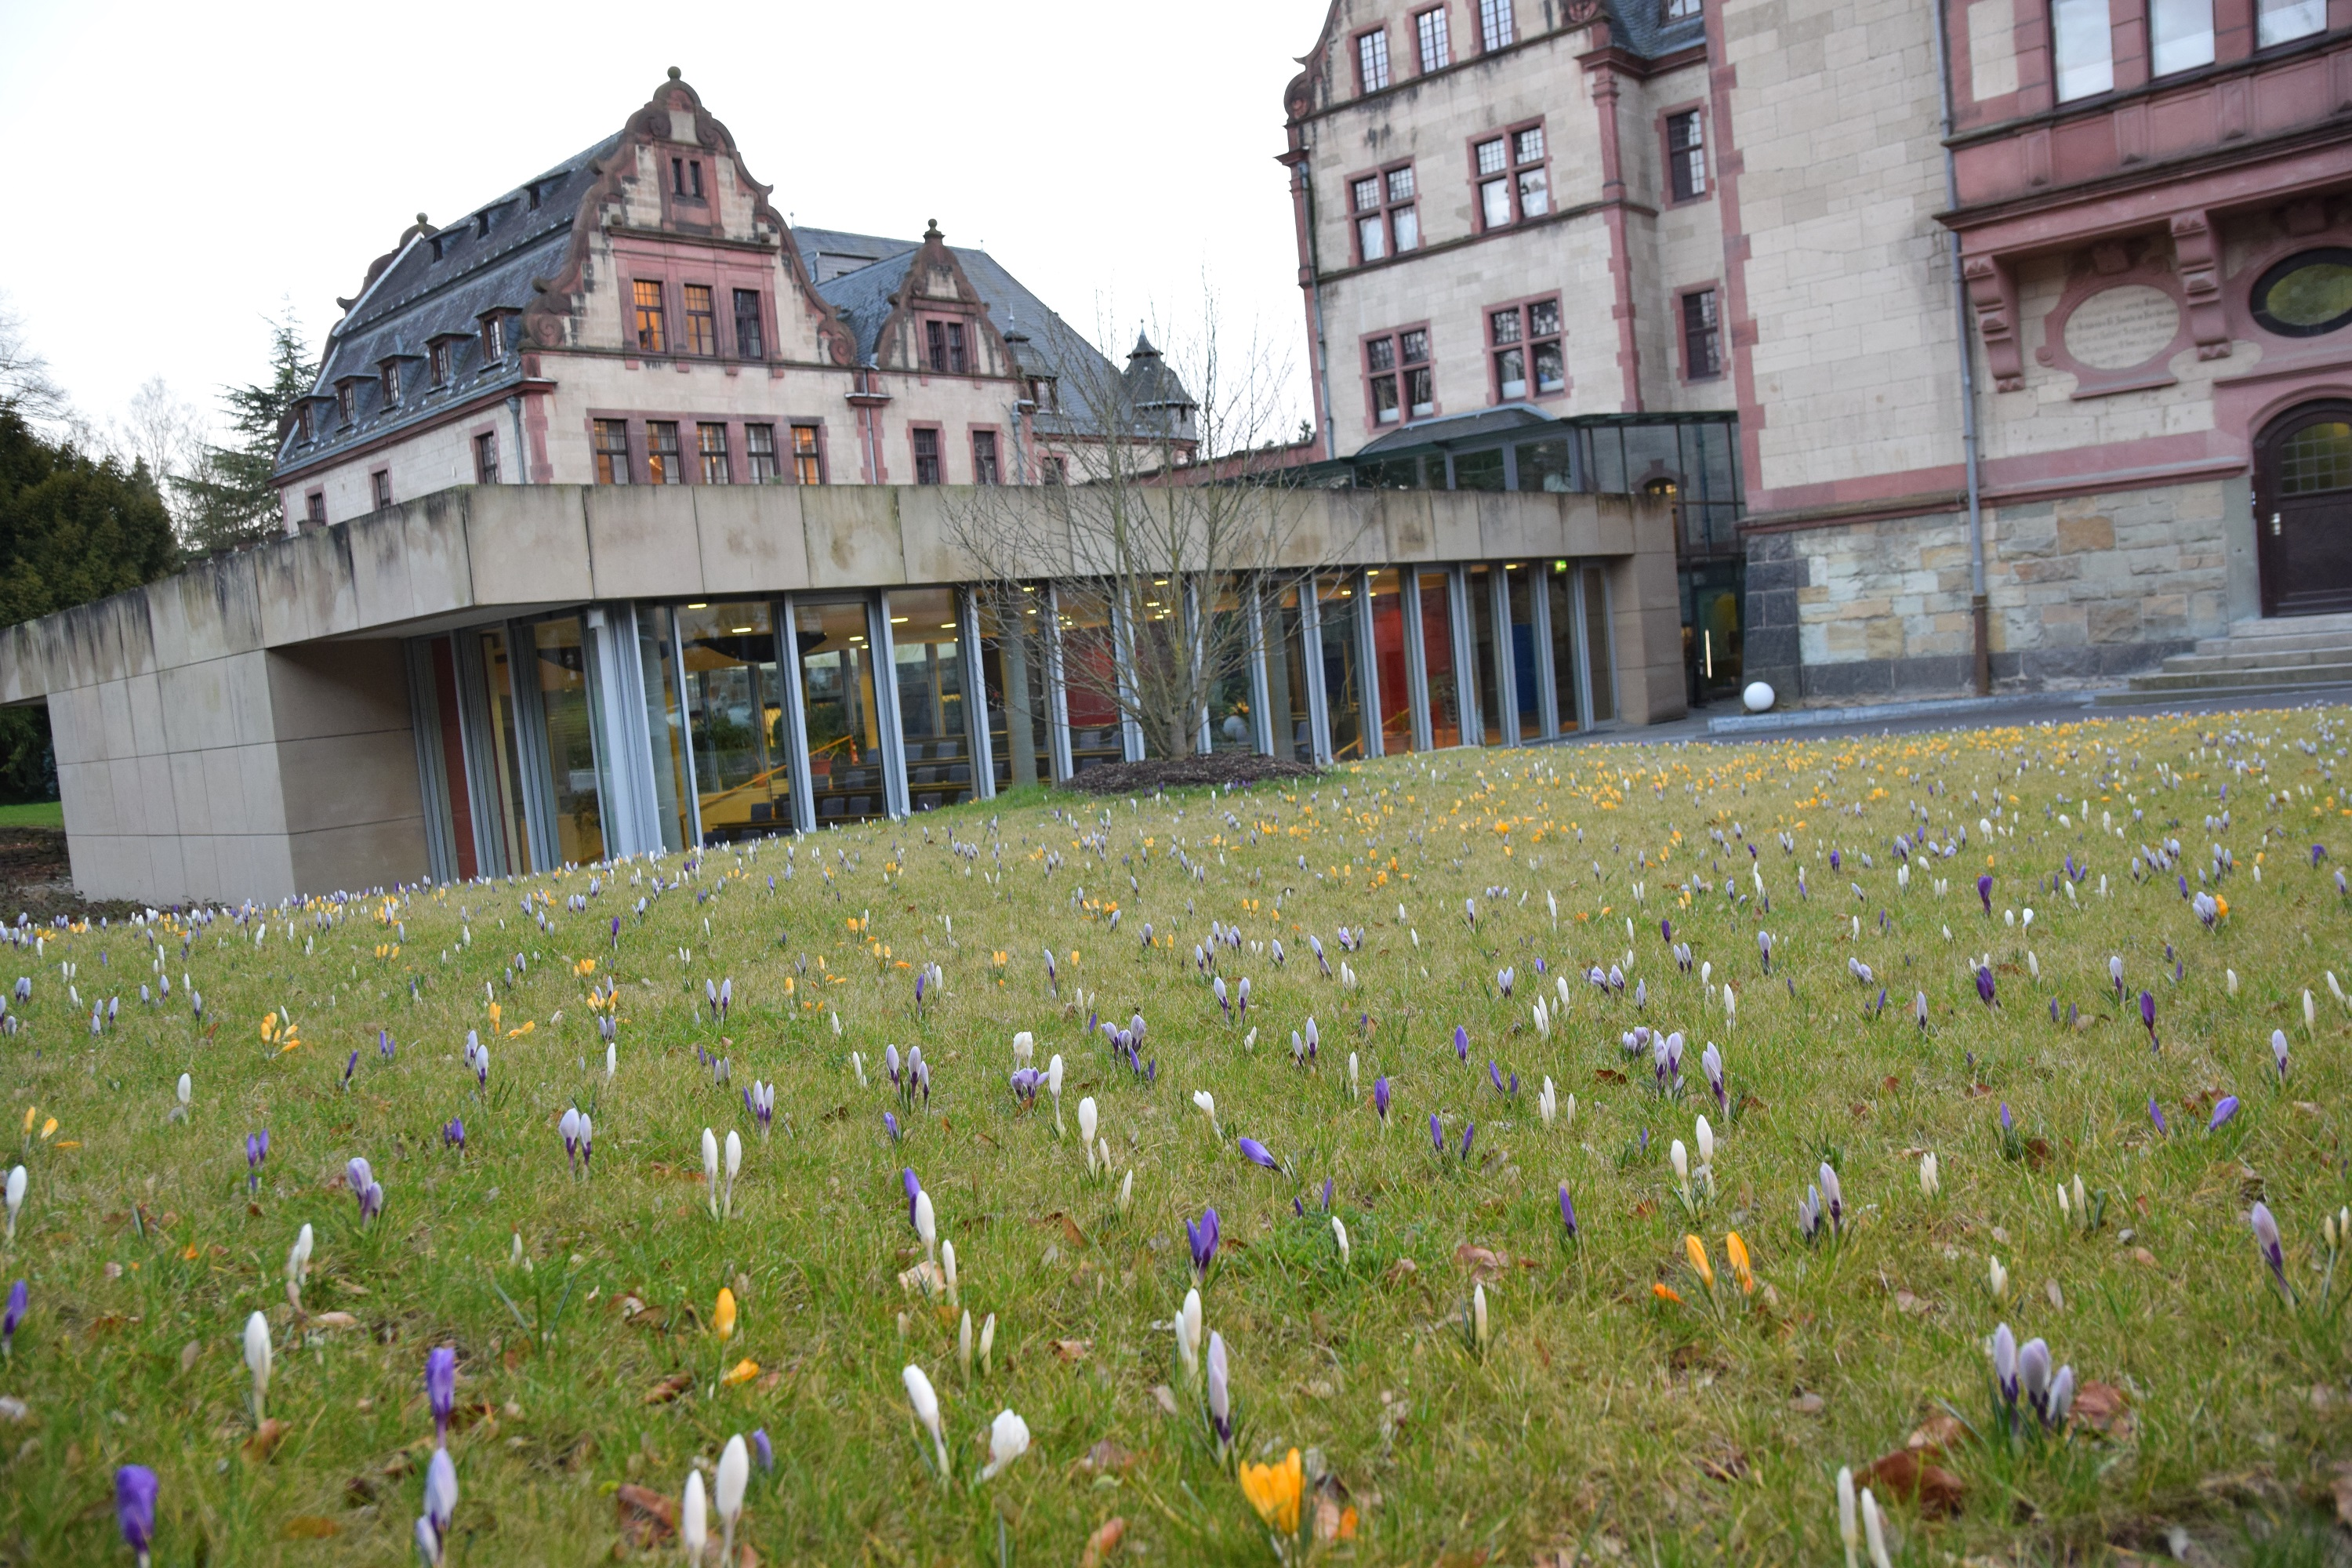
\includegraphics[width=0.49\textwidth]{figure/vereinbarkeitsworkshop_2017_PZ}\hfill
      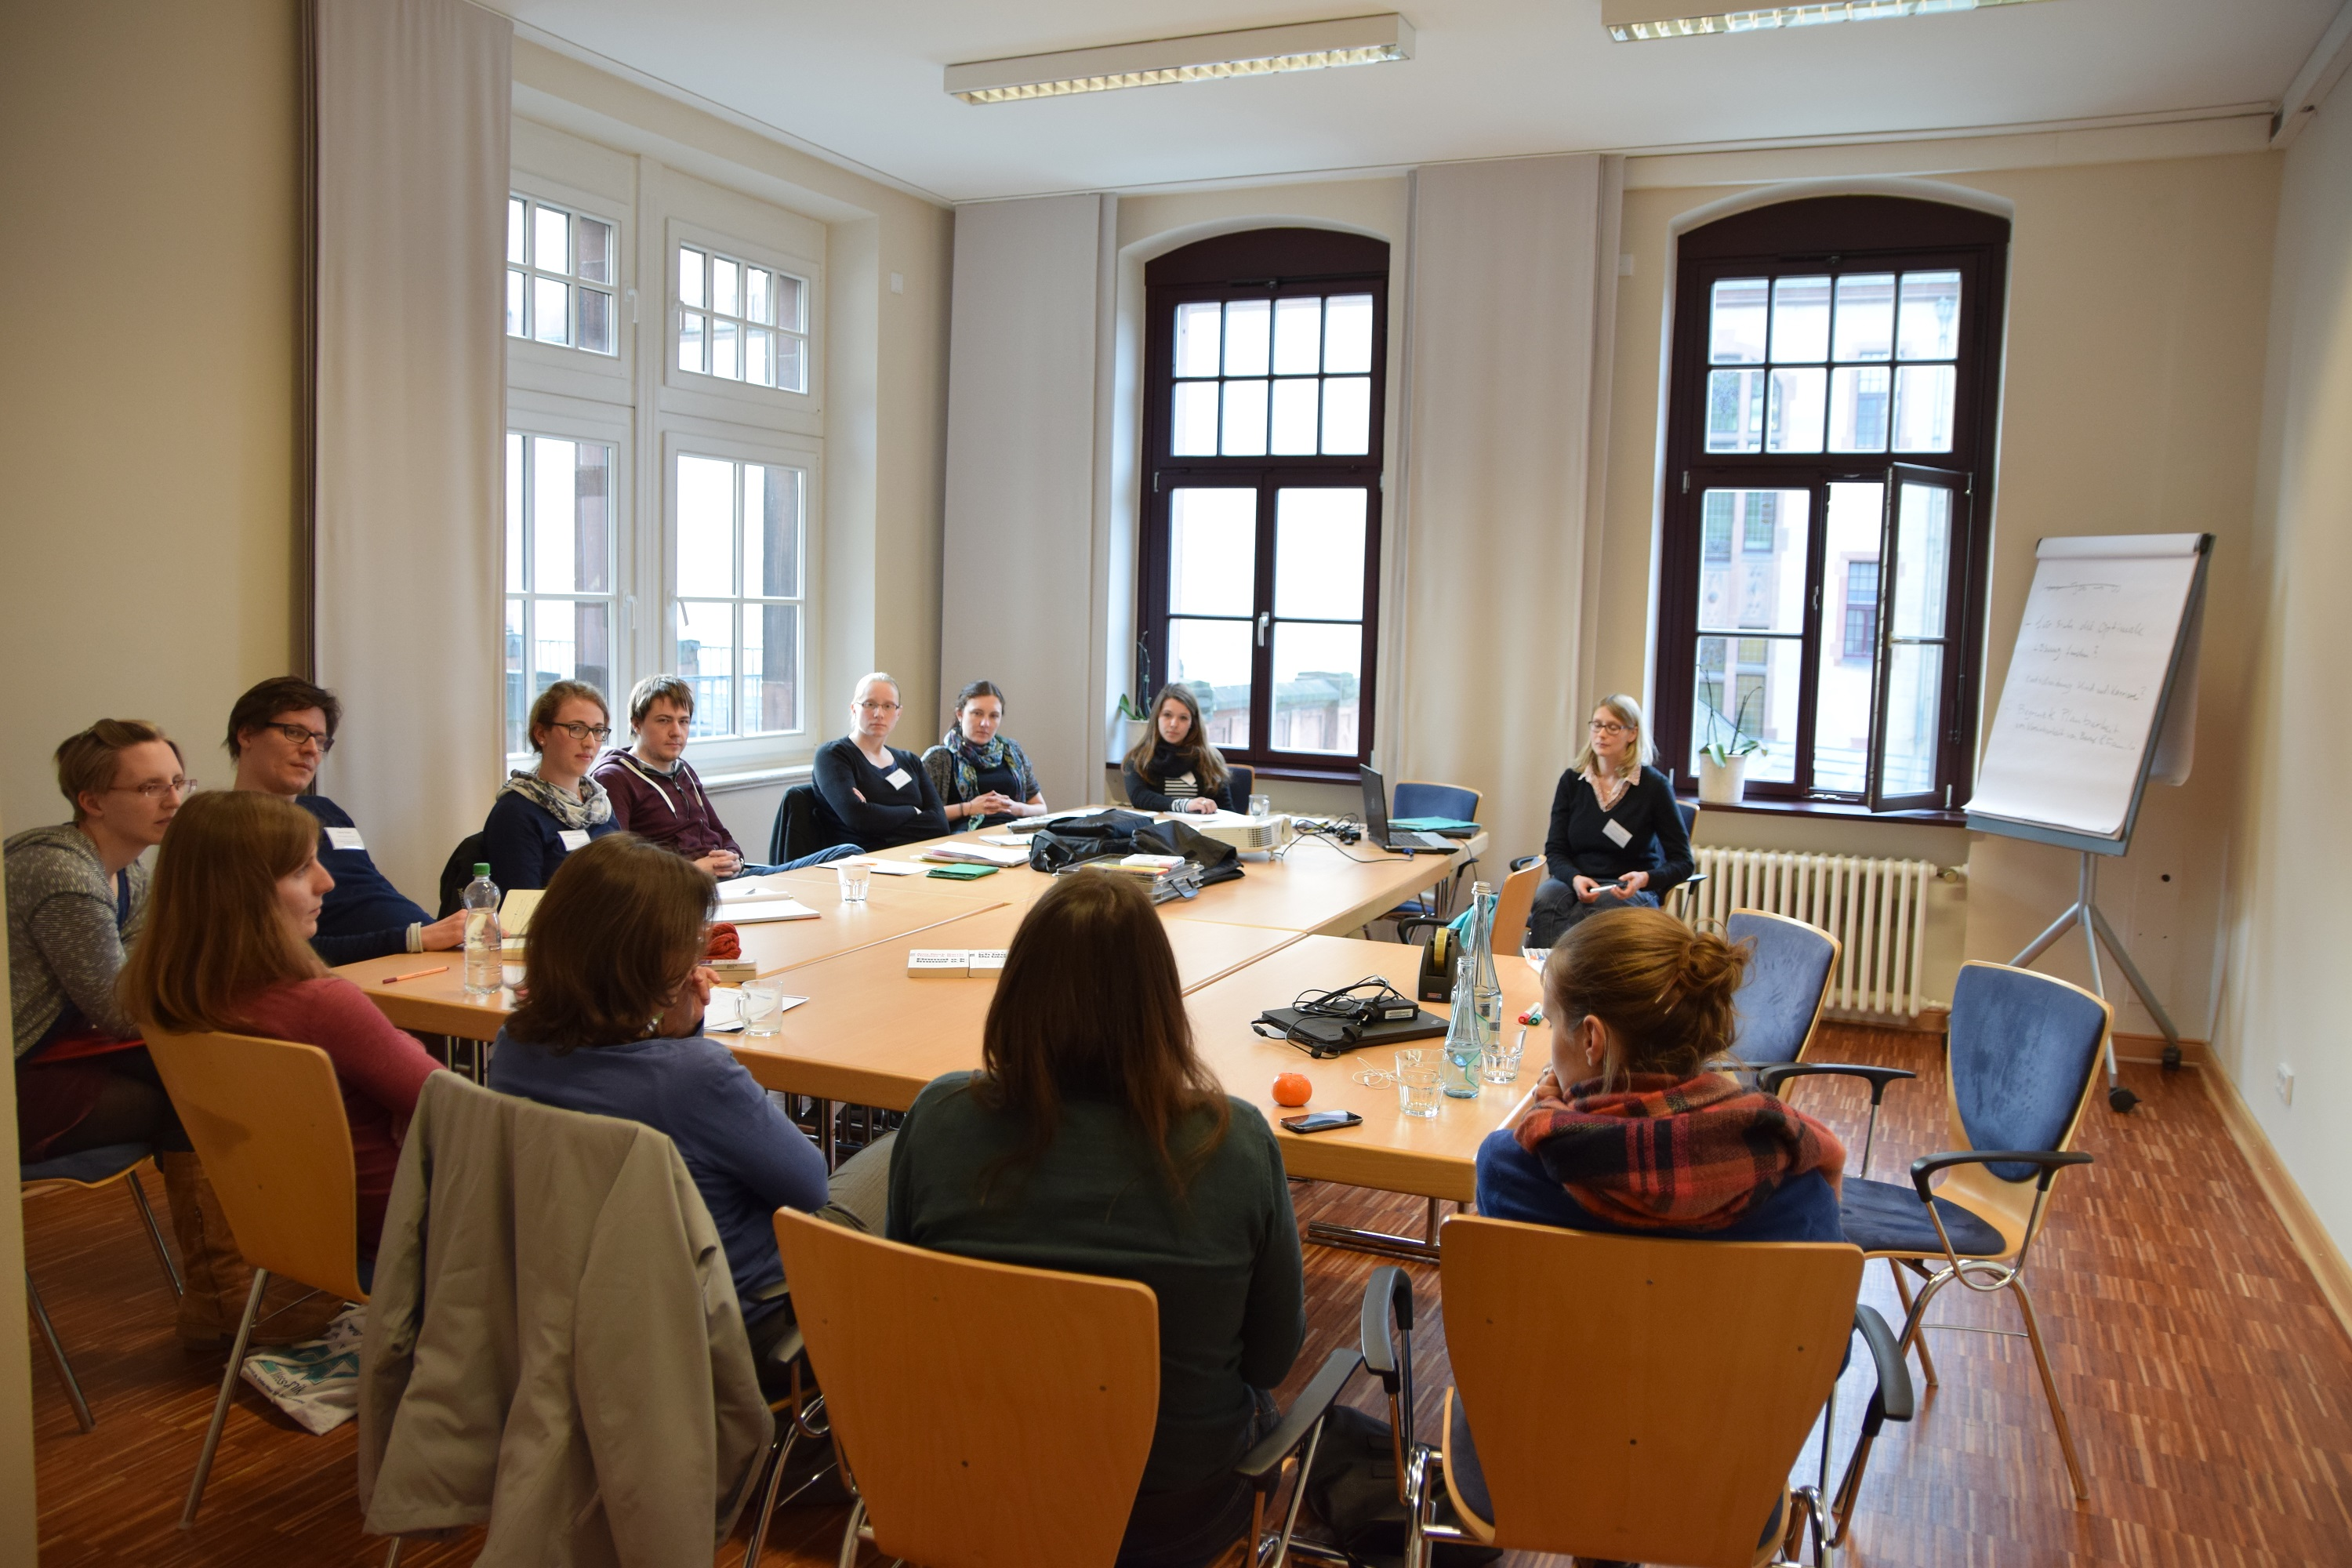
\includegraphics[width=0.49\textwidth]{figure/vereinbarkeitsworkshop_2017_TN}\\
      \begin{center}
        Vereinbarkeitsworkshop 2017 $\rightarrow$ Physikkarriere und Familie
      \end{center}
     \end{figure}
  \end{minipage}
  \begin{minipage}[0.4\textwidth]
    \begin{itemize}
      \item Berufsvorbereitungsseminare
      \item Vereinbarkeitsworkshop
    \end{itemize}
    Austausch mit Physikern über nichtphysikalisches Thema
  \end{minipage}
\end{frame}

\begin{frame}{Internationales}
  \begin{figure}
    \centering
    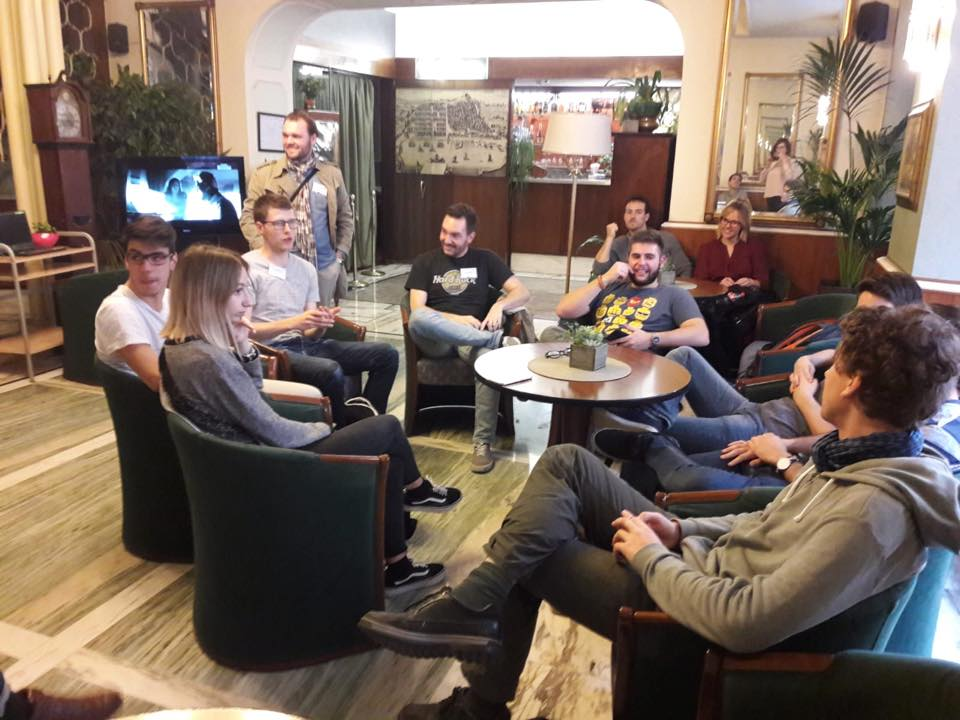
\includegraphics[width=0.6\textwidth]{figure/gipe_2018}
    \begin{center}
      Italienaustausch ( GIPE ) - AISF $\leftrightarrow$ jDPG
    \end{center}
  \end{figure}

  \begin{figure}
    \centering
    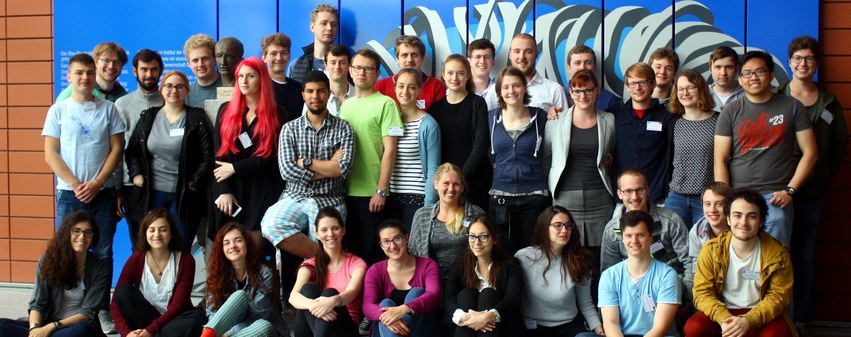
\includegraphics[width=0.6\textwidth]{figure/mafie_2017}
    \begin{center}
      Ungarnaustausch - Mafie $\leftrightarrow$ jDPG
    \end{center}
  \end{figure}
\end{frame}

\begin{frame}{"Exkursionen"}
  \begin{minipage}[0.8\textwidth]
    \begin{figure}
      \centering
      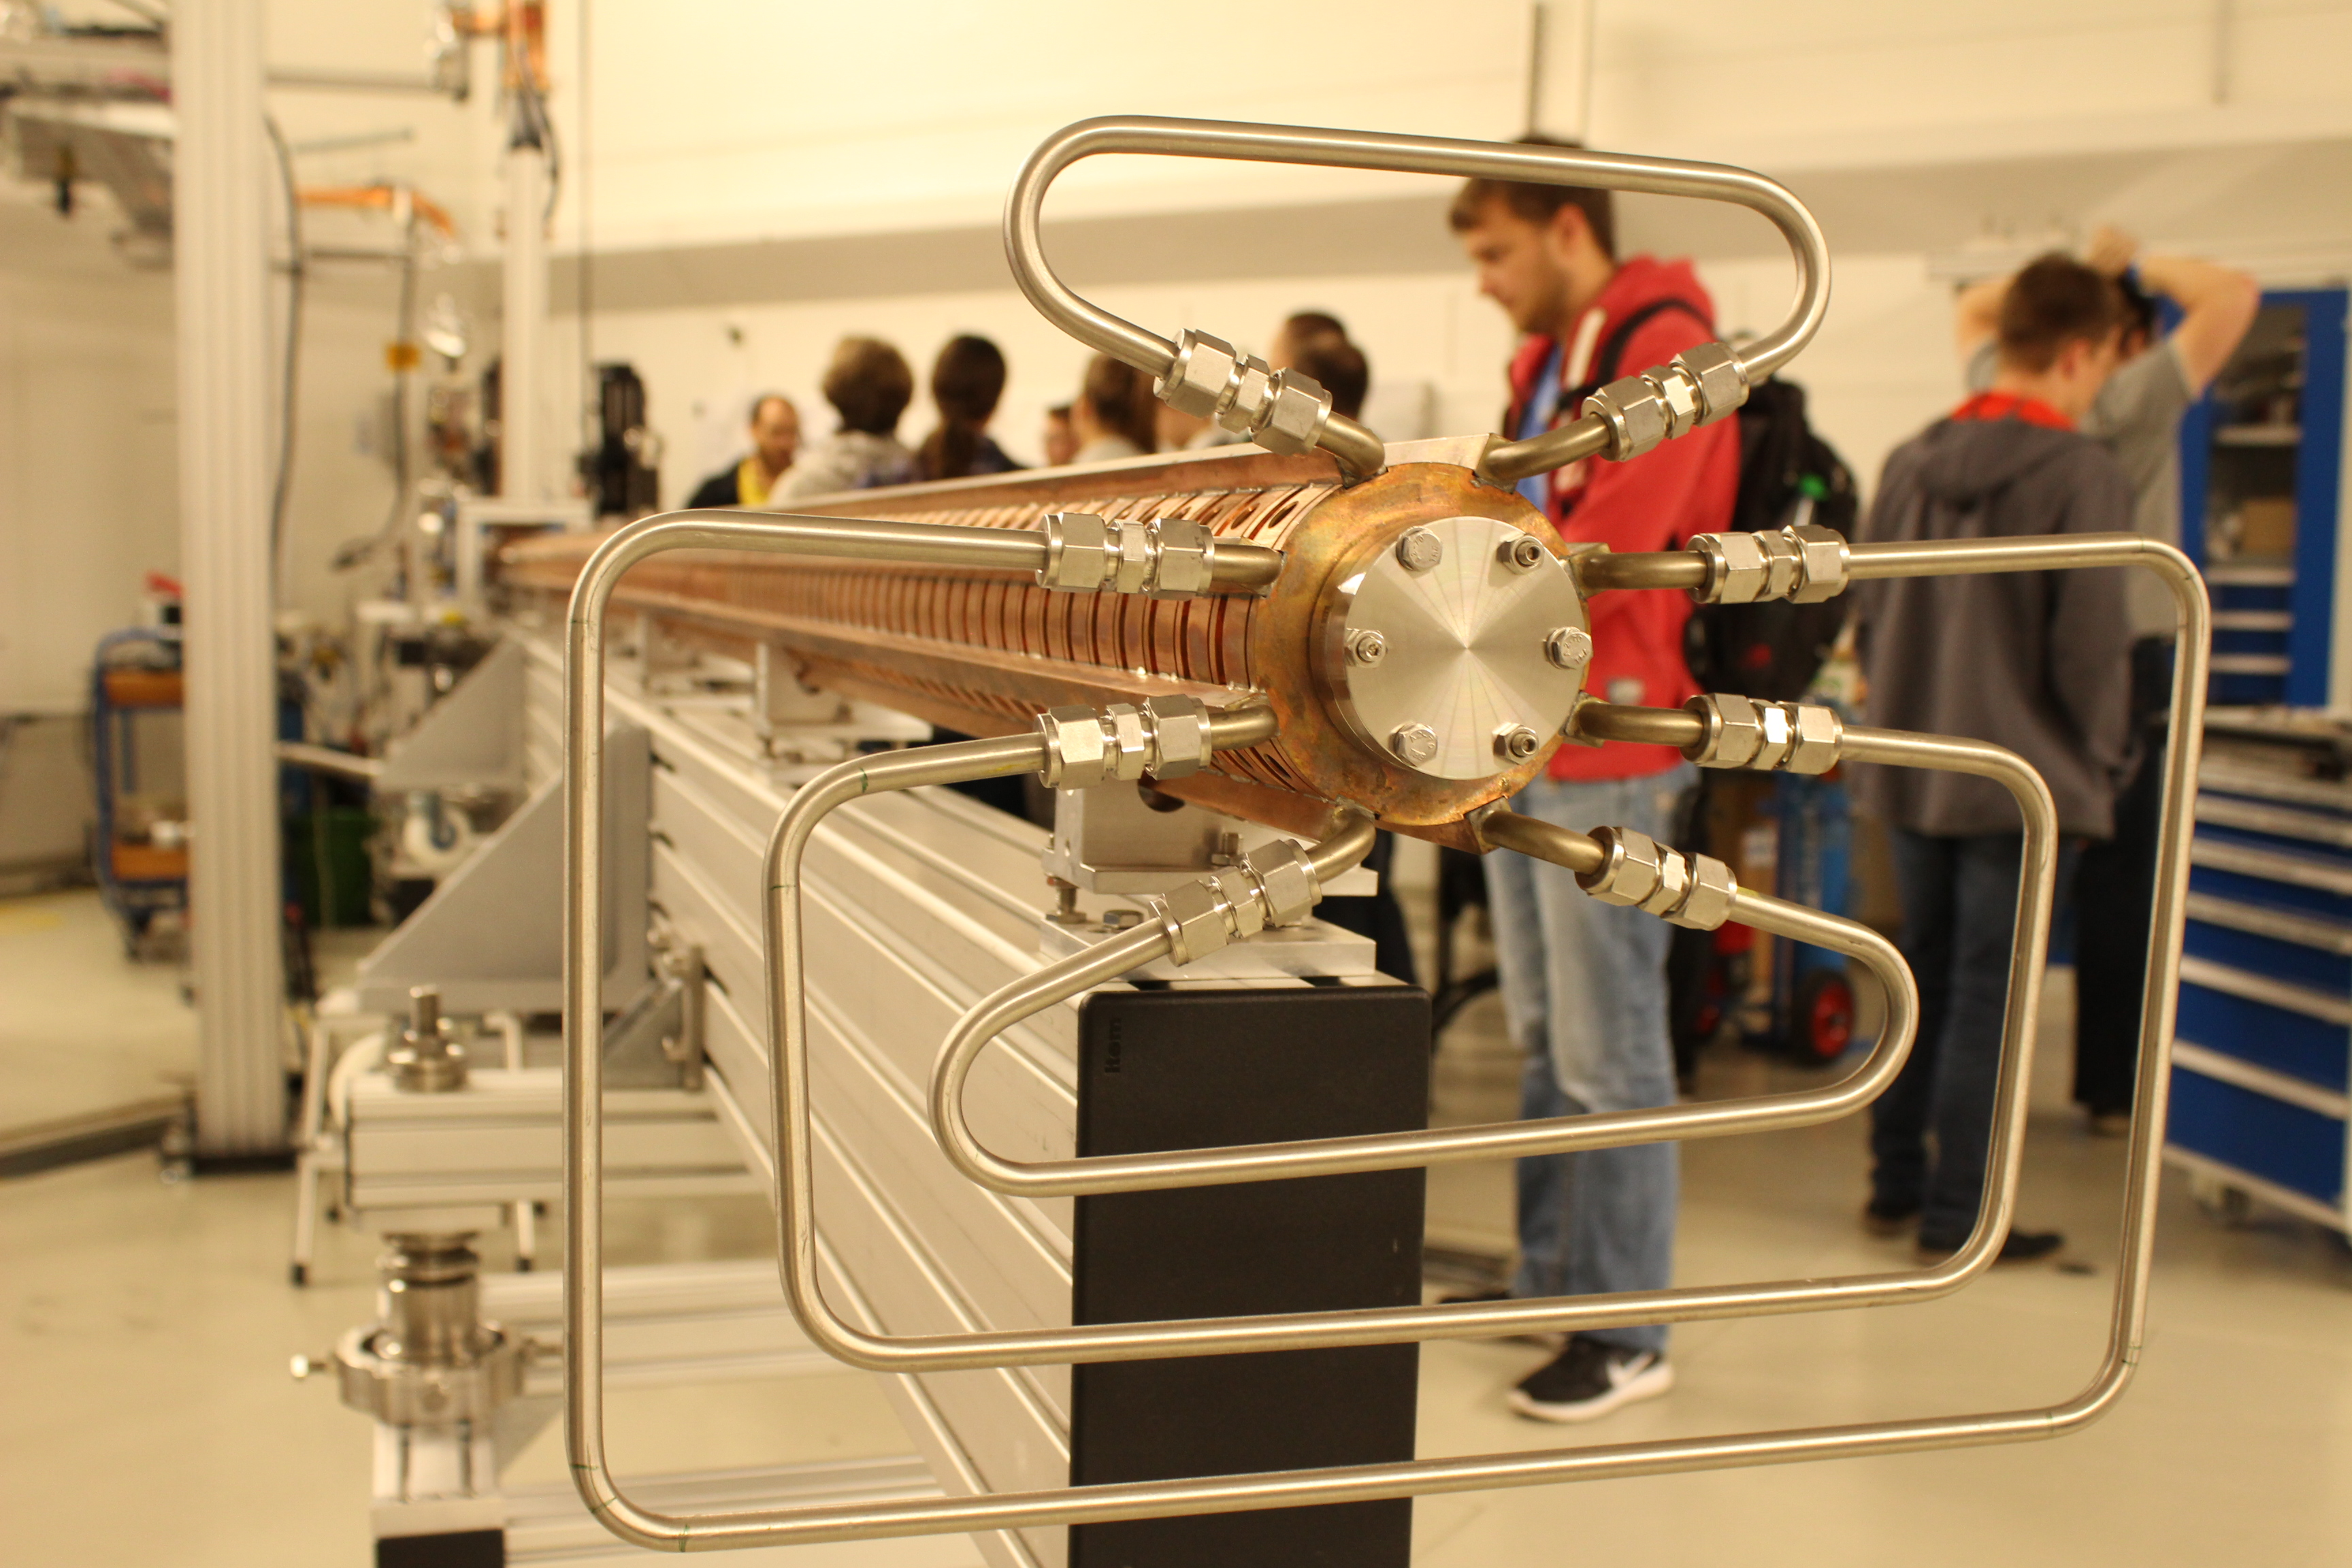
\includegraphics[width=0.6\textwidth]{figure/soex_2017}
     \end{figure}
  \end{minipage}
  \begin{minipage}[0.2\textwidth]
    \begin{itemize}
      \item Sommerexkursion
    \end{itemize}
    jDPG auf Tour - das Event zum Wiedersehen
  \end{minipage}

  \begin{minipage}[0.8\textwidth]
    \begin{figure}
      \centering
      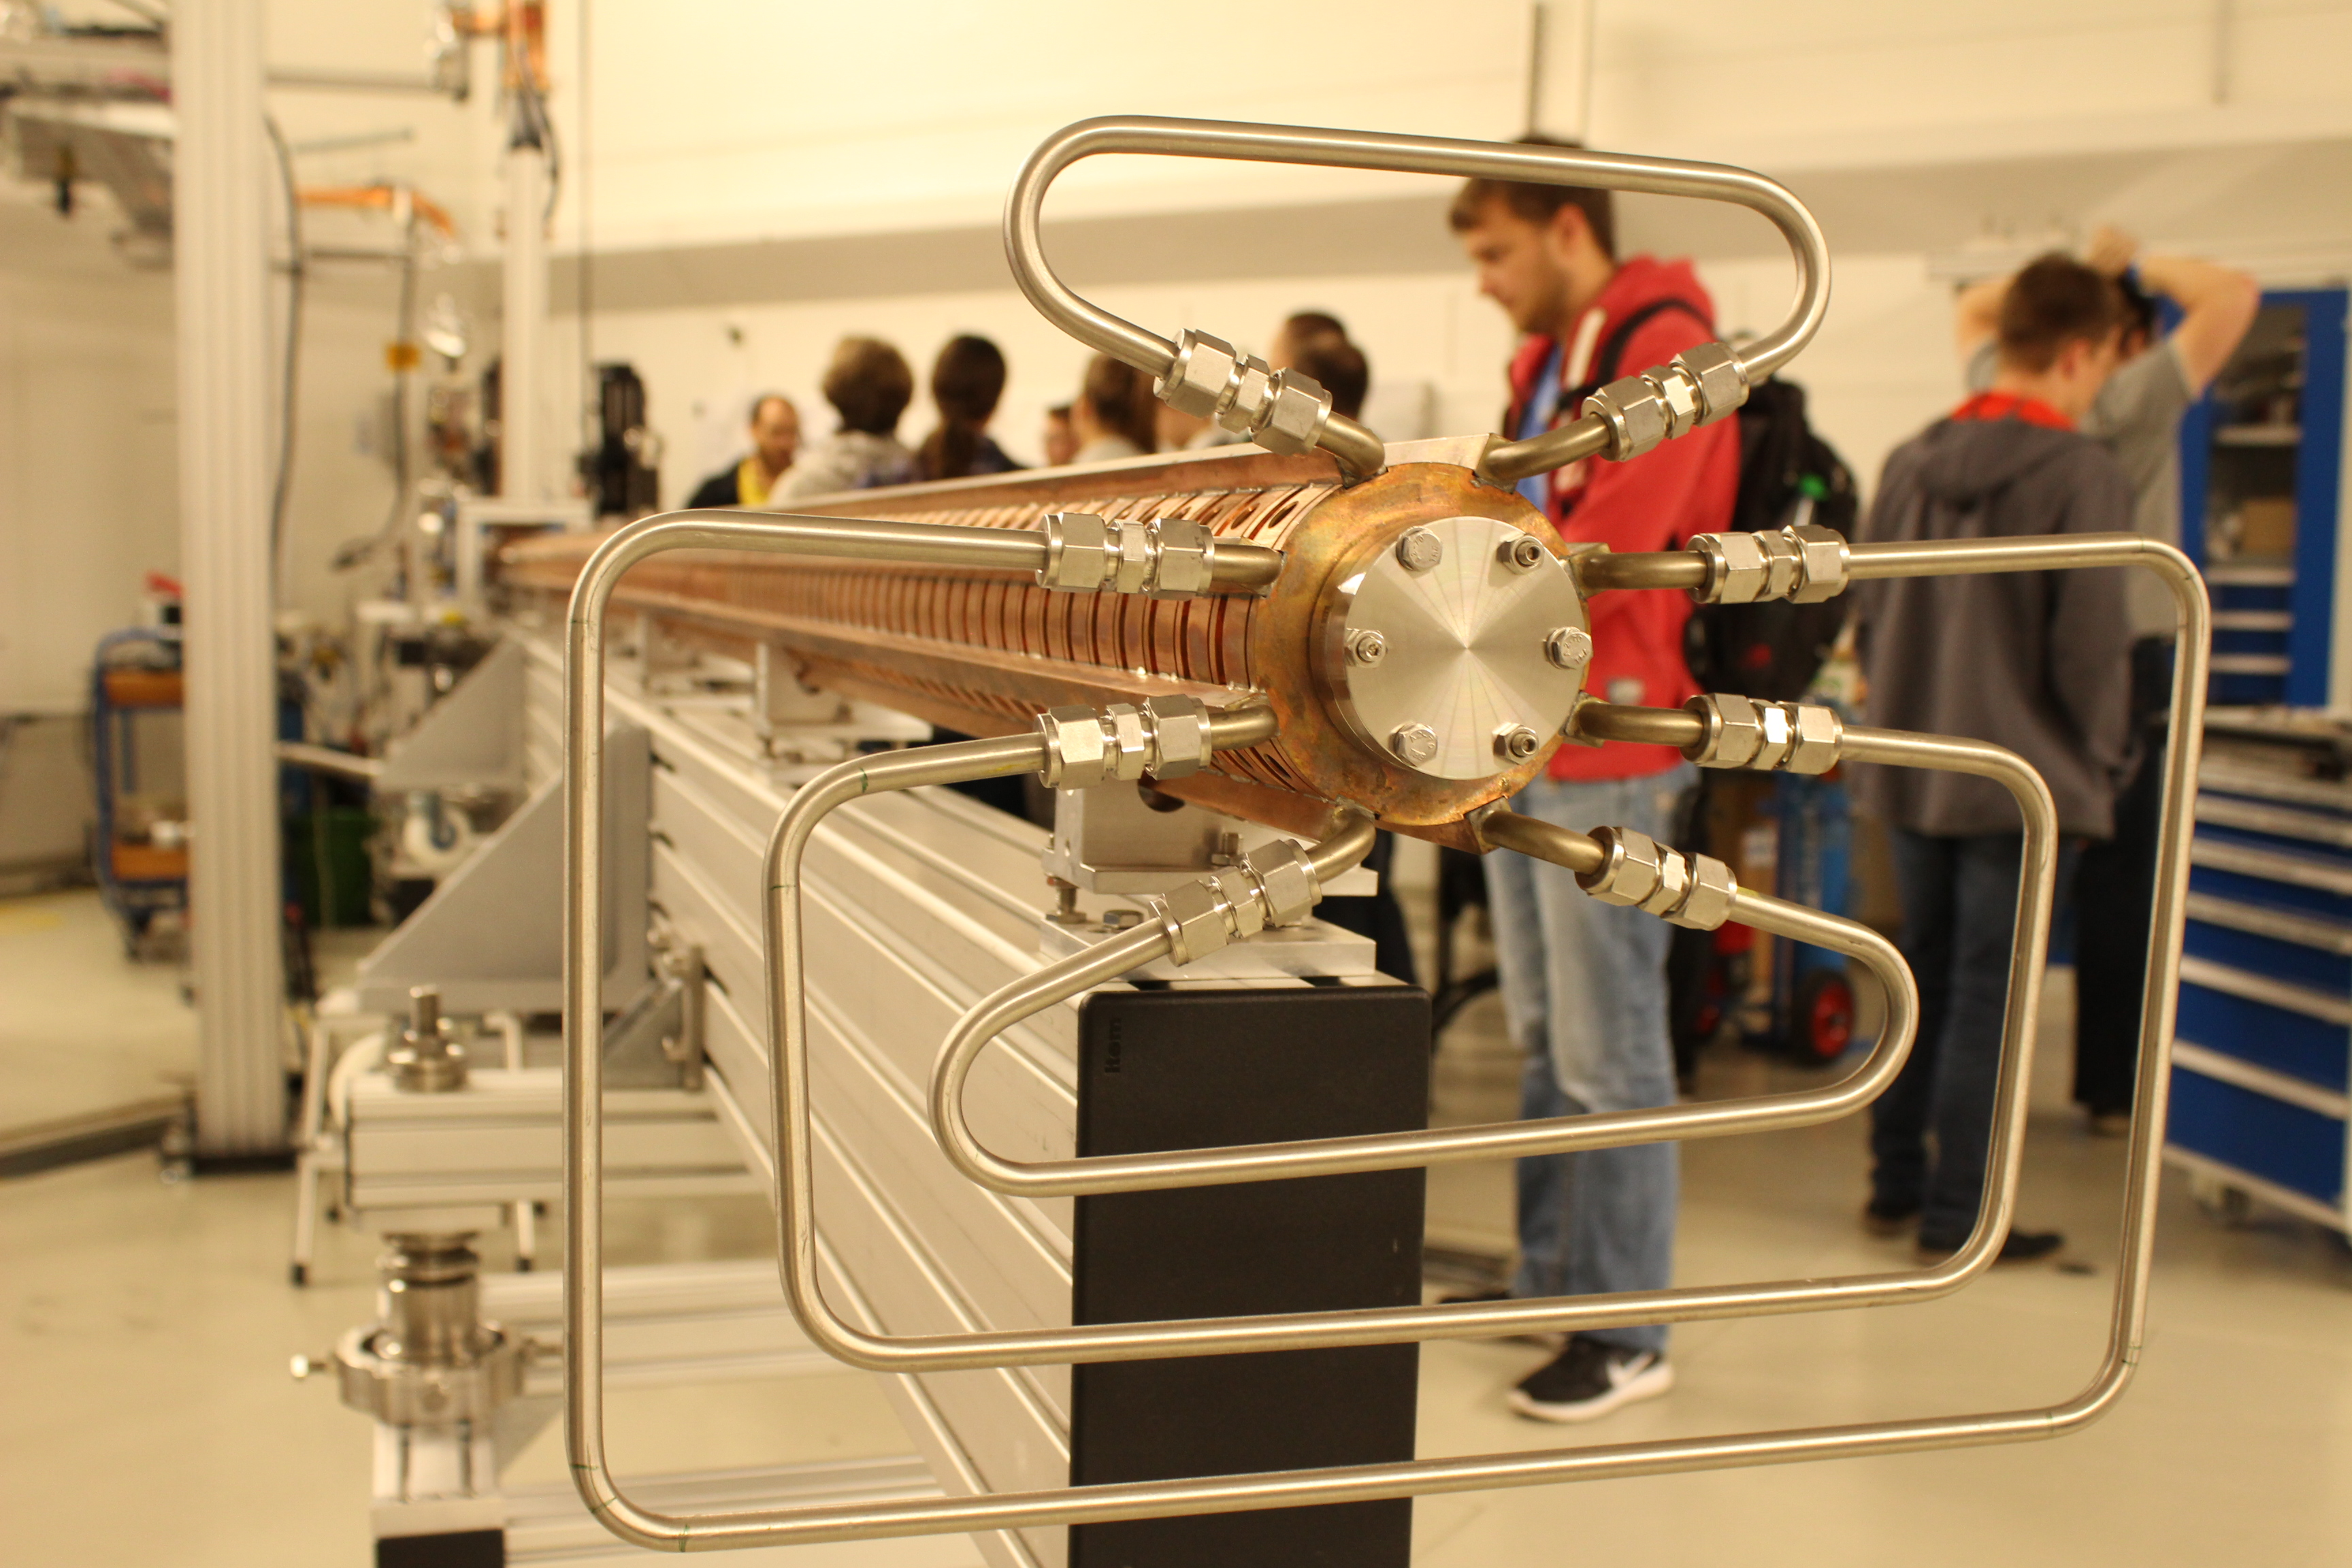
\includegraphics[width=0.6\textwidth]{figure/soex_2017}
     \end{figure}
  \end{minipage}
  \begin{minipage}[0.2\textwidth]
    \begin{itemize}
      \item Sommerexkursion
    \end{itemize}
    jDPG auf Tour - das Event zum Wiedersehen
  \end{minipage}
\end{frame}


\begin{frame}{Zusammenfassung}
  \begin{itemize}
    \item Vernetzungstreffen
    \item DOPPLERS
    \item intensives Wochenende
    \begin{itemize}
      \item BVS / PhD-BVS
      \item Wochenendseminar
      \item Theoretiker Workshop
      \item Physik trifft ...
    \end{itemize}
    \item Besichtigungen / Führungen / $\neq$ Exkursion ;)
    \begin{itemize}
      \item Sommerexkursion
      \item bundesweite Exkursion
    \end{itemize}
    \item Internationales
    \begin{itemize}
      \item Ungarn-Austausch
      \item Italien-Austausch
    \end{itemize}
  \end{itemize}
\end{frame}


%%%%%%%%%%%% Danksagung und Gruppenfoto %%%%%%%%%%%%%%%%%%%%%
\begin{frame}{Danke für eure Mitarbeit}
  \begin{center}
    {\Large Danke für eure Mitarbeit}
  \end{center}
  \begin{minipage}[c]{0.35\textwidth}
    
\includegraphics[]{figure/thank_you_1}
  \end{minipage}
  \hfill
  \begin{minipage}[c]{0.64\textwidth}
    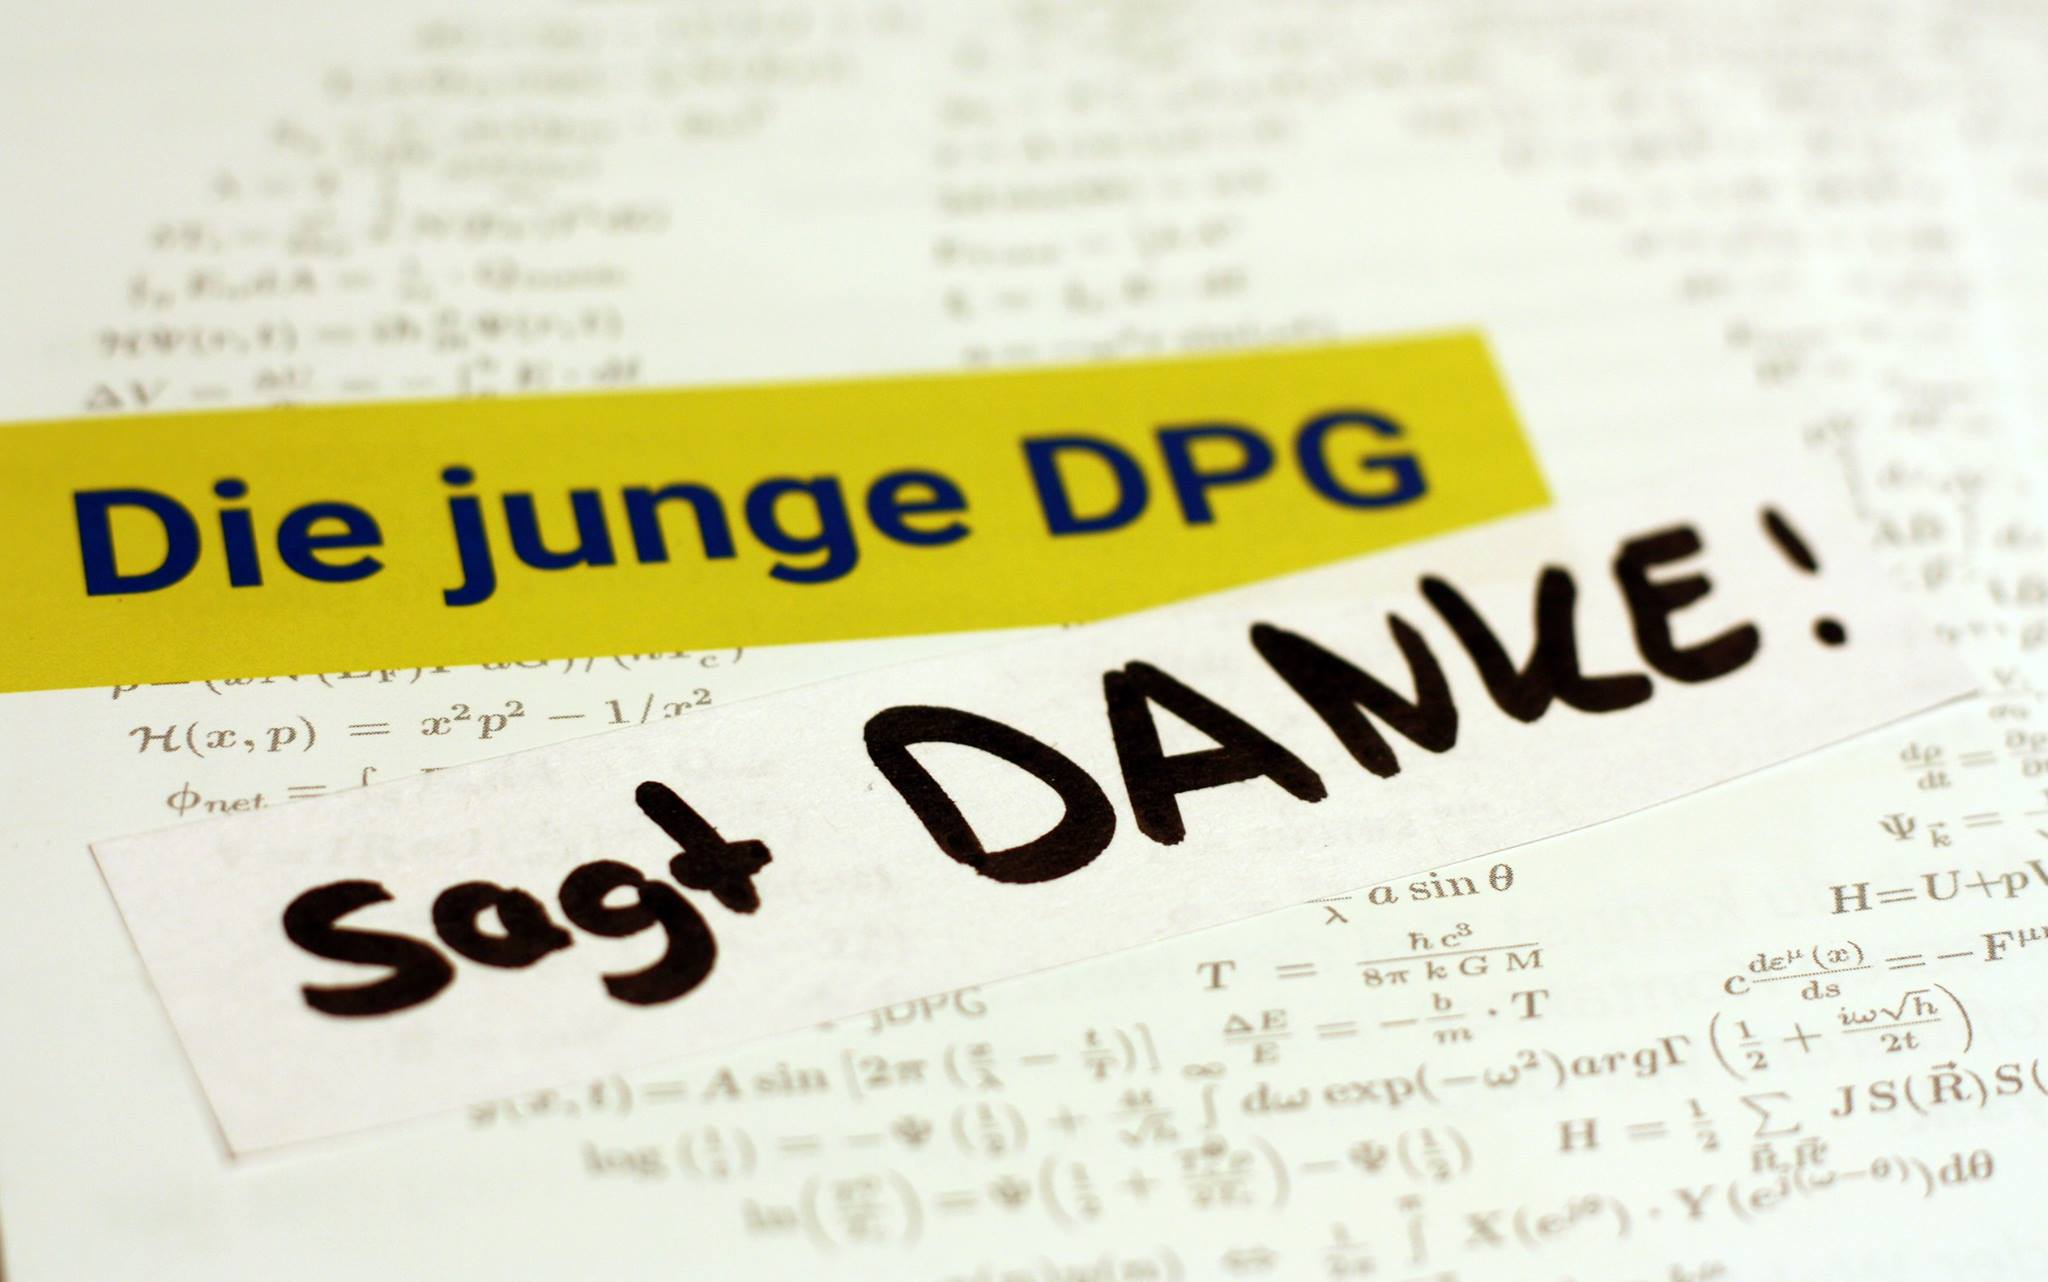
\includegraphics[width=0.99\textwidth]{figure/20171206-Christina-Nolte-Merphi}
  \end{minipage}
\end{frame}

\end{document}
